\seccion{Entrop\'ias y divergencias generalizadas}
\label{Sec:SZ:Generalizadas}

\SZ{Partout, voir convexite stricte, en 1,  idem pour h monotone, etc. vis a vis
  des cas d'egalite avec les divergences.}

A pesar de  que la entrop\'ia de Shannon y  sus cantidades asociadas demostraron
sus  potencias  tan  de un  punto  de  vista  descriptivo  que en  t\'ermino  de
aplicaciones en la  transmisi\'on de la informaci\'on y  la compresi\'on, varias
nociones  informacionales, tipo entrop\'ias  o divergencias,  aparecieron luego.
En  esta  secci\'on  no  se  desarollar\'a  todos  los  enfoques  ni  todas  las
aplicaciones  tan  la literatura  es  importante. La  meta  es  dar los  caminos
conduciendo a las generalizaciones de la entrop\'ia de Shannon por un lado, y de
la divergencia de Kullback-Leibler por  el otro lado. No son siempre vinculados,
a pesar  de que sea  deseable que a  cada entrop\'ia sean asociados  nociones de
entrop\'ias condicionales y relativas.

% ================================= Salicru

\subseccion{Entrop\'ias y propiedades}
\label{Ssec:SZ:Salicru}

% ----- Entropias generalizadas particulares
%\paragraph{Unas  primeras  generalizaciones particulares}  
Si  la entrop\'ia  de Shannon  fue el  punto de  salida fundamental  en  todo el
desarollo  de la  teor\'ia de  la  informaci\'on, un  poco m\'as  de una  decada
despu\'es  de  su  papel  clave  y  muy completo,  R\'enyi  propuso  una  medida
generalizada~\cite{Ren61}.   Su  punto  de  vista  fue  m\'as  matem\'atico  que
f\'isico o ingeniero.  Retom\'o los axiomas de Fadeev~\cite{Fad56, Fad58, Khi57}
% Feinstein, cf ref  de R��nyi
%
para  probabilidades  incompletas~\footnote{En  esta  secci\'on, los  $p_i$  son
  componentes  del  vector  $p$   no  necesariamente  asociado  a  una  variable
  aleatoria; Hay  que entender de  que $p_i =  p_X(x_i)$ si son asociados  a una
  variable aleatoria $X$.}  $p = \begin{bmatrix} p_1 & \cdots & p_n
\end{bmatrix}^t,  \quad p_i  \ge  0,  \quad w_p  =  \sum_i p_i  \le  1$: (i)  la
invarianza de  $H(p)$ por permutaci\'on de  os $p_i$, (ii) la  continuidad de la
incerteza elemental  $H(p_i)$ ($p_i$ visto como  probabilidad incompleta), (iii)
$H\left( \frac12 \right) = 1 $,  (iv) la aditividad $H(p \otimes q) = H(p)+H(q)$
donde $p \otimes  q$ es el producto de  Kronecker o tensorial~\footnote{Ver nota
  de    pie~\ref{foot:MP:Kronecker}   pagina~\pageref{foot:MP:Kronecker}},   \ie
probabilidad conjunta de dos variables independientes, y consider\'o en lugar de
la recursividad  un axioma  dicho de  valor promedio, axioma  muy parecido  a la
recursividad. Para $p$ \ y \ $q$ probabilidades incompletas tales que $p \, \cup
\, q = \begin{bmatrix} p_1 & \cdots  & p_n & q_1 & \cdots & q_m \end{bmatrix}^t$
sea incompleta  ($w_p +  w_q \le  1$), el  axioma (v) es  $H(p \,  \cup \,  q) =
\frac{w_p \, H(p) +  w_q \, H(q)}{w_p + w_q}$.  Demostr\'o que  con (v) en lugar
de la recursividad,  el conjunto de axiomas conduce de nuevo  a la entrop\'ia de
Shannon.  La generalizaci\'on propuesta por R\'enyi era de generalizar el axioma
(v) reemplazando la media aritm\'etica por una media generalizada (v') $H^\ren(p
\, \cup  \, q)  = g^{-1}  \left( \frac{w_p \,  g\big( H^\ren(p)  \big) +  w_q \,
    g\big( H^\ren(q) \big)}{w_p +  w_q}\right)$ con $g$ estrictamente mon\'otona
y  continua,  llamado  media  {\it  cuasi-aritm\'etica,  o  cuasi-lineal,  o  de
  Kolmogorov-Nagumo}.       De     las      propiedades     de      la     media
cuasi-aritm\'etica~\cite{Nag30,  Kol30, Kol91, HarLit52},  eso es  equivalente a
buscar una entrop\'ia elemental $H^\ren(p_i)$ y reemplazar la media aritm\'etica
\ $\sum_i  p_i H^\ren(p_i)$ por  una media de Kolmogorov-Nagumo,  $g^{-1} \left(
  \sum_i p_i g\big( H^\ren(p_i)  \big) \right)$.  R\'enyi propus\'o la funci\'on
de  Kolmogorov-Nagumo \  $g_\lambda(x) =  2^{(\lambda-1) x},  \quad  \lambda >0,
\quad \lambda  \ne 1$, probando  de que los axiomas  (i)-(ii)-(iii)-(iv)-(v') se
cumplen, conduciendo  a la  entrop\'ia de R\'enyi  de un vector  de probabilidad
$p$,
%
\[
H_\lambda^\ren(p) =  \frac{1}{1-\lambda} \log_2 \left(  \sum_{i=1}^n p_i^\lambda
\right)
\]
%
\noindent  Relaxando   el  axioma  (iii),   se  puede  elegir   $g_\lambda(x)  =
a^{(\lambda-1) x}, \quad a  > 0, \quad a \ne 1$; el  logaritmo ser\'a de la base
$a$ cualquiera. En  lo que sigue, usaremos $\log$ sin  precisar la elecci\'on de
base.   R\'enyi nombr\'o  esta  medida  de incerteza  {\it  entrop\'ia de  orden
  $\lambda$}. Notablemente,
%
\[
H_1^\ren(p)  \equiv   \lim_{\lambda  \to  1}  H_\lambda^\ren(p)   =  H(p)  \quad
\mbox{entrop\'ia de Shannon}
\]
%
\noindent En otros t\'erminos, la clase de R\'enyi contiene como caso particular
la  entrop\'ia de  Shannon.   En su  papel,  R\'enyi introdujo  una ganancia  de
informaci\'on,  parecida  a una  entrop\'ia  relativa,  probando  que las  solas
entrop\'ias admisibles son  la de Shannon y la que  introdujo.  Volveremos en la
secci\'on siguiente  sobre esta entrop\'ia  relativa, o divergencia  de R\'enyi.
Por          axiomas,          las         propiedades~\ref{Prop:SZ:continuidad}
(continuidad),~\ref{Prop:SZ:permutacion}    (invarianza    por    permutaci\'on)
y~\ref{Prop:SZ:aditividad}  (additividad)   de  la  entrop\'ia   de  Shannon  se
conservan entonces en el marco de R\'enyi y se pierde~\ref{Prop:SZ:recursividad}
(recursividad), todav\'ia por axiomas. Veremos luego la otras que se conservan o
modifican en un marco m\'as general.

Unos a\~nos  despu\'es de R\'enyi, de  la famosa escuela  matem\'atica checa, J.
Havrda   \&    F.    Charv\'at   en~\cite{HavCha67}    (ver   tambi\'en~\cite[en
checo]{Vaj68}) volvieron a los axiomas de Khintchin, para extender la entopia de
Shannon,  \ie  considerando  (i)   la  invarianza  por  permutaci\'on,  (ii)  la
continuidad, (iii) la expansividad, (iv) $H^\hc(1) = 0$ y $H^\hc\left( \frac12 ,
  \frac12   \right)  =   1$,  pero   generalizando  la   recursividad   por  (v)
$H^\hc(p_1,\ldots,p_n)   =   H^\hc(p_1,\ldots,p_{n-2},p_{n-1}+p_n)   +   \lambda
(p_{n-1}+p_n)^\lambda         H^\hc\left(        \frac{p_{n-1}}{p_{n-1}        +
    p_p},\frac{p_n}{p_{n-1} + p_p} \right),  \quad \lambda > 0$~\footnote{En sus
  papel, lo imponen  para cualquier par $(p_i, p_j)$  sin imponer la invarianza
  por permutaci\'on, pero es equivalente  a la exposici\'on de este p\'arrafo.}.
Con $\lambda = 1$ se recupera la recursividad estandar, pero con $\lambda \ne 1$
eso permite dar un  peso diferente a la incerteza del estado  interno, \ie a las
probabilidades  que  se juntan  (la  describen  como clasificaci\'on  refinada).
Estos axiomas conducen necesariamente a la entrop\'ia (teorema~1 del papel)
%
\[
H_\lambda^\hc(p) = \frac{1}{1-2^{1-\lambda}} \left( 1 - \sum_i p_i^\lambda \right)
\]
%
que  nombraron {\it  $\lambda$-entrop\'ia structural}.   De nuevo,  relaxando el
axioma  (iv),   se  puede  reemplazar  en  el   coeficient  $2^{1-\lambda}$  por
$a^{1-\lambda}, \quad a > 0, \quad a \ne 1$. De nuevo, aparece que la entrop\'ia
de Shannon es un caso particular,
%
\[
H_1^\hc(p)  \equiv   \lim_{\lambda  \to   1}  H_\lambda^\hc(p)   =   H(p)  \quad
\mbox{entrop\'ia de Shannon}
\]
%
Por axioma, se conservan las propiedades~\ref{Prop:SZ:continuidad} (continuidad)
y~\ref{Prop:SZ:expansabilidad}  (expansabilidad) de  Shannon en  este  marco. Se
prob\'o tambi\'en que se conserva la  propiedad de concavidad con respecto a los
$p_i$~\ref{Prop:SZ:concavidad},   la   de   maximalidad~\ref{Prop:SZ:cotamaxima}
alcanzada para una distribuci\'on uniforma (teorema~2). Aun que no aparece as\'i
en        el        papel,        satisface        la        propiedad        de
Schur-concavidad~\ref{Prop:SZ:Schurconcavidad}  (teorema~3).   A  pesar  de  que
mencionan que $H_\lambda^\hc$ sea diferente de $H_\lambda^\ren$, es sencillo ver
que hay un mapa uno-uno entre las dos entrop\'ias.  Se mencionar\'an en un marco
m\'as general otras propiedades de esta entrop\'ia.

Independiente de Havrda  \& Charv\'at, de la escuela h\'ugara  de teor\'ia de la
informaci\'on,  Z.  Dar\'oczy  en~\cite{Dar70}  defin\'o la  entrop\'ia $H^f$  a
partir de una {\it funci\'on  informaci\'on} $f$ satifaciendo (i) $f(0) = f(1)$,
(ii) $f\left(\frac12\right) = 1$ \ y  la ecuaci\'on funcional (ii) $f(x) + (1-x)
f\left(  \frac{y}{1-x} \right)  = f(y)  + (1-y)  f\left(  \frac{x}{1-y} \right)$
sobre  $\{  (x,y)  \in [0  ;  1)^2,  \quad  x+y  \le  1 \}$,  siendo  $H^f(p)  =
\sum_{i=2}^n s_i  f\left( \frac{p_i}{s_i} \right), \quad  s_i = \sum_{j=1}^{i-1}
p_j$.   Dar\'oczy mostr\'o  que  si $f$  es medible,  o  continua en  $0$, o  no
negativa  y  acotada, necesariamente  $f(x)  =  h_2(x) =  -x  \log_2  x -  (1-x)
\log_2(1-x)$,   conduciendo  a   la  entrop\'ia   de  Shannon   (teorema~1;  ver
tambi\'en~\cite{Lee64, Tve58,  Ken64}).  En otros  t\'erminos, su axioma  (v) es
alternativa a la recursividad.  Para  extender la entrop\'ia de Shannon, propuso
extender  este   axioma  (v)  por   la  ecuaci\'on  funcional   $f_\lambda(x)  +
(1-x)^\lambda   f_\lambda\left(   \frac{y}{1-x}   \right)   =   f_\lambda(y)   +
(1-y)^\lambda   f_\lambda\left(   \frac{x}{1-y}   \right)$,   lo   que   condujo
necesariamente a la entrop\'ia (teoremas~2 y~3)
%
\[
H_\lambda^\dar(p) = \frac{1}{1-2^{1-\lambda}} \left( 1 - \sum_i p_i^\lambda \right)
\]
%
\noindent  es decir  nada  m\'as que  la  entrop\'ia introducida  por Havdra  \&
Charv\'at. En lo  que sigue, se la denotar\'a  $H_\lambda^\hcd$. Sin embargo, el
estudio  de  Dar\'oczy  fue m\'as  intensivo  que  el  de Havdra  \&  Charv\'at.
Primero, not\'o  el mapa entre su  entrop\'ia y la de  R\'enyi. Adicionalmente a
Havdra-Charv\'at prob\'o que  se conserva la propiedad~\ref{Prop:SZ:permutacion}
(invarianza  por   permutaci\'on,  que  no   era  un  axioma  en   su  enfoque),
$H_\lambda^\hcd\left( \frac12 , \frac12 \right) = 1$ (lo llama normalizaci\'on),
la  expansividad~\ref{Prop:SZ:expansabilidad},  una  aditividad  extendida,  una
recursividad extendida precisamente  del modelo de Havrda-Charv\'at (teorema~4).
Prob\'o  tambi\'en~\ref{Prop:SZ:positividad}, positividad  alcanzado en  el caso
determinista  y  la  maximalidad~\ref{Prop:SZ:cotamaxima}  en el  caso  uniforme
(teorema~6), que  incidentalmente $H_\lambda^\hcd\left( \frac1\alpha  , \ldots ,
  \frac1\alpha \right)$ crece con el  cardinal $|\X| = \alpha$.  Muy interesante
tambi\'en es se puede definir una  entrop\'ia condicional en el mismo modelo que
en  el  caso  de  Shannon  $H_\lambda^\hcd(X|Y)  =  \sum_y  \left[  p_{X|Y}(x,y)
\right]^\lambda  H_\lambda^\hcd( p_{X|Y}(\cdot,y)  )$, que  existe una  regla de
cadena~\ref{Prop:SZ:cadena},   $H_\lambda^\hcd(X,Y)    =   H_\lambda^\hcd(Y)   +
H_\lambda^\hcd(X|Y)$ y que condicionar reduce la entrop\'ia $H_\lambda^\hcd(X|Y)
\le    H_\lambda^\hcd(X)$    (teorema~8)~\ref{Prop:SZ:condicionar}.     Mostr\'o
tambi\'en que  si se  pierde la aditividad,  se obiene para  \ $X$  \ e \  $Y$ \
independientes \ $H_\lambda^\hcd(X,Y)  = H_\lambda^\hcd(X) + H_\lambda^\hcd(Y) +
\left(  2^{1-\lambda}  -  1  \right) H_\lambda^\hcd(X)  H_\lambda^\hcd(Y)$.   La
propiedades de regla  de cadena le permiti\'o revisitar  la caracterisaci\'on de
un canal de transmisi\'on y  redefinir una capacidad canal extendidas (capacidad
tipo $\lambda$;  basicamente se  usa el mismo  enfoque que Shannon,  pero usando
$H_\lambda^\hcd$ en lugar de $H$, ver secci\'on~6 del papel).

% ----- Entropias generalizadas h,phi
%\paragraph{Una  clase m\'as  general  y sus  propiedades}

\

Las entrop\'ias  tipo Havdra-Charv\'at-Dar\'oczy fueron  (re)descubiertos varias
otras  veces  y/o estudiadas  m\'as  detenidamente  en  varios campos  y  varios
extensiones fueron  introducidas~\cite[entre otros]{Var66, Oni66,  Kap67, Vaj68,
  LinNie71,  Ari71,  Bur72,   AczDar75,  ShaMit75,  ShaMit75,  ShaTan75,  Mit75,
  BoeLub80, Fer80, Tsa88, Rat91, Kan01, Bec09}.  Un primer enfoque m\'as general
es debido a  S.  Arimoto en los primeros a\~nos  de la decada 1970~\cite{Ari71}.
Fue rediscubierto  y estudiado  con m\'as detalles  una decada despu\'es  por J.
Burbea y C.  R.  Rao~\cite{BurRao82} y luego por M.  Salicr\'u~\cite{Sal87} o M.
Teboulle~\cite{Teb92}   entre  otros.    La  medida   propuesta,   llamada  {\it
  $\phi$-entrop\'ia}, es definida por
%
\[
\hphi[p]  =   -\sum_i  \phi(p_i)  \qquad   \mbox{con}  \qquad  \phi   \:  \mbox{
  estrictamente convexa}
\]
%
Burbea  y  Rao  asociaron una  medida  de  divegencia  a esta  entrop\'ia.   Las
$\phi$-entrop\'ias  contienen Shannon como  caso particular  ($\phi(x) =  x \log
x$),  as\'i que  la clase  de Havdra-Charv\'at-Dar\'oczy  ($\phi(x) =  \frac{x -
  x^\lambda}{2^{1-\lambda}-1}$) como mencionado, pero no la clase de R\'enyi. De
hecho, las  $\phi$-entrop\'ias se  enmarcan en una  clase un poco  m\'as amplia,
llamada {\it  $(h,\phi)$-entrop\'ias}~\cite{SalMen93, MenMor97}. Cambiamos ac\`a
substancialmente su escritura  de la literatura por razones  de homogeneidad con
la    $\phi$-entrop\'ia   (y    las   divergencias    que    se   introducir\'an
luego)~\footnote{En  la literatura,  no hay  el signo  $-$, y  hay  que invertir
  c\'oncava y convexa.}
%
\begin{definicion}[$(h,\phi)$-entrop\'ia]\label{Def:SZ:HPhiEntropia}
  La $(h,\phi)$-entrop\'ia de una  distribuci\'on de probabilidad $p_X$ definida
  sobre $\X$ de cardinal finito $|\X| = \alpha$ es definida por
  %
  \[
  \hhphi[X] = \hhphi[p_X] = h\left(  - \sum_{x \in \X} \phi\left( p_X(x) \right)
  \right)
  \]
  %
  donde o
  %
  \begin{itemize}
  \item $\phi$ \ es estrictamente convexa y \ $h$ \ creciente, o
  \item $\phi$ \ es estrictamente c\'oncava y \ $h$ \ decreciente
  \end{itemize}
  %
  Frecuentemente, se supone adicionalmente que  $\phi$ y $h$ son de clase $C^2$,
  que $\phi(0) = 0$ (la incerteza elemental asociada a un estado de probabilidad
  nula vale cero) y, sin perdida de generalidad, que $h(-\phi(1)) = 0$.
\end{definicion}
%
\noindent  (ver  tambi\'en~\cite{Est97}  para  una  generalizaci\'on  aun  m\'as
amplia). Cu\'ando $h(x) = x$  se recupera la $\phi$-entrop\'ia, incluyendo la de
Shannon y las de Havdra-Charv\'at-Dar\'oczy. Adem\'as, la familia de R\'enyi cae
tamb\'ien en  esta familia  ($\phi(x) = -  x^\lambda$ \  y \ $h(x)  = \frac{\log
  x}{1-\lambda}$)  as\'i que  todas  las entrop\'ias  evocadas  en el  p\'arrafo
anterior.

Como   en   el   caso   de    Shannon,   para   $X   =   (X_1,\ldots,X_d)$,   la
$(h,\phi)$-entrop\'ia de $X$ es una $(h,\phi)$-entrop\'ia conjunta de los $X_i$.

Obviamente, de  las propiedades  de la entrop\'ia  de Shannon, se  conservan las
propiedades~\ref{Prop:SZ:continuidad}    (continuidad),~\ref{Prop:SZ:permutacion}
(invariaza    por   permutaci\'on),~\ref{Prop:SZ:biyeccion}    (invarianza   por
transformaci\'on       biyectiva      de      $X$),~\ref{Prop:SZ:expansabilidad}
(expansabilidad, debido a $\phi(0) = 0$).

Adem\'as  se conserva  la  Schur-concavidad \ con una reciproca:
%
\begin{propiedadesPhi}\setcounter{enumi}{\value{PropSchurConcavidad}}
%
\item Schur-convavidad:
  %
  \[
  p \prec q \quad \Longleftrightarrow \quad \hhphi[p] \ge \hhphi[q] \quad \forall \:
  (h,\phi)
  \]
  %
  % \centerline{Reciprocamente,  si $\quad \forall \:  (h,\phi), \quad \hhphi[p]
  %   \ge \hhphi[q] \quad \mbox{ entonces } \quad p \prec q$}
  %
  En otros t\'erminos,  se obtiene la relaci\'on de  mayorisaci\'on si se cumple
  la  relaci\'on  de ordre  entr\'opicas  para  \underline{todos}  los pares  de
  funciones entr\'opicas  $(h,\phi)$.  La  Schur-concavidad (y su  reciproca) es
  consecuencia     de     la     desigualdad     de     Schur~\cite{Sch23}     o
  Hardy-Littlewood-P\'olya~\cite{HarLit29,   HarLit52}  o  Karamata~\cite{Kar32}
  (ver   tambi\'en~\cite[Cap.~3,  Prop.~C.1   \&   Cap.~4,  Prop.~B.1]{MarOlk11}
  o~\cite[Teorema~II.3.1]{Bha97}): $p \prec q \: \Rightarrow \: \sum_i \phi(p_i)
  \le \sum_i \phi(q_i)$ para toda funci\'on $\phi$ convexa, y reciprocamente.
\end{propiedadesPhi}
% Schur, I.  (1923). Issai Schur Collected  Works (A.  Brauer  and H.  Rohrbach,
% eds.), Vol. II. pp. 416����427. Springer-Verlag, Berlin, 1973]
%
%
% Ver Schur-Ostrowski f  sym, Schur-convexe ssi (xi - xj)  (df/dx_i - df/dxj) \ge
% 0, 1 \le i \ne j \le alpha
%
Como consecuencia, se  conservan la positividad~\ref{Prop:SZ:positividad} gracia
a \ $\phi(0) = 0$ \ y \ $h(-\phi(1)) = 0$ \ (alcanzado en el caso determinista),
la maximalidad~\ref{Prop:SZ:cotamaxima} (caso uniforme),
%
\[
0 \le \hhphi[p_X] \le h\left( - \alpha \, \phi\left( \frac1\alpha \right) \right)
\]
%
as\'i que
%
\[
\hhphi[\begin{bmatrix}  \frac1\alpha &  \cdots  & \frac1\alpha  \end{bmatrix}^t]
\quad \mbox{funci\'on creciente de } \alpha
\]

Con respecto a la concavidad~\ref{Prop:SZ:concavidad}, no se conserva en general:
%
\begin{propiedadesPhi}\setcounter{enumi}{\value{PropConcavidad}}
\item\label{Prop:SZ:concavidadHPhi} Si $h$ es c\'oncava, entonces $\hhphi[p]$ es
  c\'oncava con  respecto a $p$.   Eso es una  consecuencia de la  concavidad de
  $\phi$ y  decrecencia de $h$ (resp.  convexidad/crecencia)  conjuntamente a la
  concavidad de $h$.  La reciproca no  es verdad.  Por ejemplo, se puede ver que
  si $\lambda  < 1$, la  entrop\'ia de R\'enyi  es c\'oncava, pero se  proba que
  existe  un  $\lambda^*(\alpha)  >  1$  tal que  para  cualquier  $\lambda  \le
  \lambda^*(\alpha)$  se conserva  la  concavidad, a  pesar  de que  $h$ no  sea
  necesariamente c\'oncava~\cite[p.~57]{BenZyc06}.
\end{propiedadesPhi}

Se pierde la propiedad de recursividad~\ref{Prop:SZ:recursividad}, pero se puede
vincular  la  entrop\'ia  total con  la  obtenida  juntando  dos estados  por  una
desigualdad:
%
\begin{propiedadesPhi}\setcounter{enumi}{\value{PropRecursividad}}
\item  Sean \  $X$  \ definido  sobre  \ $\X$  \  y \  $\widebar{X}$  \ sobre  \
  $\widebar{X}$,
  %
  \[
  \left\{  \begin{array}{l}\widebar{\X}  = \{  x_1  ,  \ldots  , x_{\alpha-2}  ,
      \widebar{x}_{\alpha-1}\} \quad \mbox{con el estado interno} \quad
      \widebar{x}_{\alpha-1}   =  \{   x_{\alpha-1}  ,   x_\alpha  \},\\[2.5mm]
      p_{\widebar{X}}(x_i) = p_X(x_i), \quad 1 \le i \le \alpha-1 \quad \mbox{y}
      \quad p_{\widebar{X}}(\widebar{x}_{\alpha-1}) = p_X(x_{\alpha-1}) +
      p(x_\alpha)  \quad  \mbox{distribuci\'on  sobre  }  \widebar{\X}\\[2.5mm]
      \displaystyle   \widebar{q}(x_j)  =   \frac{p_X(x_j)}{p_X(x_{\alpha-1})  +
        p_X(x_\alpha)},  \quad j =  \alpha-1, \alpha  \quad \mbox{distribuci\'on
        del estado interno}\end{array}\right.
  \]
  %
  \[
  \hhphi[p_X] \ge \hhphi[p_{\widebar{X}}]
  \]
  %
  Esta  desigualdad es  consecuencia de  la desigualdad  de Petrovi\'c~\cite[43,
  Teorema~8.7.1]{Kuc09}, $\phi(a + b) \ge \phi(a) + \phi(b)$ para $\phi$ convexa
  y que se cancela en 0 (y  la conversa en el caso c\'oncavo), conjuntamente con
  $h$ creciente  (resp.  decreciente).   Aparte en  el caso de  Shannon y  el de
  Havdra-Charv\'at-Dar\'oczy, no hay  ning\'un v\'inculo explicito general entre
  $\hhphi[p_X]$ \ y \ $\hhphi[p_{\widebar{X}}]$.
\end{propiedadesPhi}

Se  conserva  la  super-aditividad~\ref{Prop:SZ:superaditividad}. De  hecho,  si
$\phi$ es convexa (resp.  c\'oncava) con \  $\phi(0) = 0$, \ $\forall \: 0 \le a
\le 1,  \: \phi(a u) =  \phi(a u + (1-a)  0) \le a  \phi(u)$ (resp.  desigualdad
reversa).   Entonces,  \   $\phi\left(  p_{X,Y}(x_i,y_j)  \right)  =  \phi\left(
  p_{X|Y}(x_i,y_j)  p_Y(y_j)  \right)  \le  p_{X|Y}(x_i,y_j)  \phi\left(p_Y(y_j)
\right)$, \ \ie \ $\sum_{i,j} \phi\left( p_{X,Y}(x_i,y_j) \right) \le \sum_{i,j}
p_{X|Y}(x_i,y_j) \phi\left(p_Y(y_j) \right) = \sum_i \phi\left(p_Y(y_j) \right)$
\  (resp.   desigualdad  reversa).   Se   cierra  la  prueba  con  la  crecencia
(resp. decrecencia) de $h$.


Sin  embargo, en  general, se  pierden  las propiedades~\ref{Prop:SZ:aditividad}
(aditividad), y~\ref{Prop:SZ:subaditividad}  (sub-aditividad). En particular, se
conserva solamente en el caso Shannon:
%
\begin{teorema}
  Sea $p_{X,Y}$ distribuci\'on conjunta  de variables aleatorias discretas \ $X$
  \ y \ $Y$ \ y \ $p_X$ \ y \ $p_Y$ \ las de \ $X$ \ y de \ $Y$ (marginales).
%
\[
\hhphi[p_{X,Y}]  \: \le  \: \hhphi[p_X  \otimes  p_Y] \quad  \forall \:  p_{X,Y}
\qquad \Longleftrightarrow \qquad \phi(x) = x \log x
\]
%
\ie $\hhphi$ es una funci\'on creciente de la entrop\'ia de Shannon
\end{teorema}
%
\begin{proof}
  La    reciproca     de    este    teorema    es    nada     m\'as    que    la
  propidad~\ref{Prop:SZ:subaditividad} con  el hecho de que $h$  es creciente en
  este caso.

  A continuaci\'on, la parte directa se demuestra en dos etapas:
  %
  \begin{itemize}
  \item Con  un caso particular  sobre $\X$  e $\Y$ de  cardenal 3 cada  unos se
    proba  de que  la desigualdad  no se  puede cumplir,  salvo si  la funci\'on
    entr\'opica $\phi'$ satisface a una ecuaci\'on funcional.
  %
  \item la sola soluci\'on admisible de esta ecuaci\'on se reduce a $\phi(x) = -
    x \ln x$.
  \end{itemize}
  %
  {\bf Etapa 1}: Sea el vector de probabildad
  %
  \[
  p_{X,Y}  =  p_X  \otimes   p_Y  -  c  \begin{bmatrix}  1\\-1\\0  \end{bmatrix}
  \otimes  \begin{bmatrix} 1\\-1\\0 \end{bmatrix}  \qquad \mbox{con}  \qquad p_X
  = \begin{bmatrix} a \\ \tilde{a} \\ 1-a-\tilde{a} \end{bmatrix} \quad \mbox{y}
  \quad p_Y = \begin{bmatrix} b \\ \tilde{b} \\ 1-b-\tilde{b} \end{bmatrix}
  \]
  %
  donde $(a,\tilde{a},b,\tilde{b}) \in D_{a,\tilde{a},b,\tilde{b}}$,
  %
  \[
  D_{a,\tilde{a},b,\tilde{b}} = \{  a, v, s, t:  \quad 0 < a,s <  1 \quad \wedge
  \quad 0 < v \le 1-a \quad \wedge \quad 0 < t \le 1-s \}
  \]
  %
  y \ $c \in C_{a,\tilde{a},b,\tilde{b}}$,
  %
 \[
  C_{a,\tilde{a},b,\tilde{b}} = \big[ - 1 + \max\big\{ a b , \tilde{a} \tilde{b}
  , 1 - a \tilde{b} , 1 - \tilde{a}  b \big\} \, , \, \min\big\{ a b , \tilde{a}
  \tilde{b} , 1 - a \tilde{b} , 1 - \tilde{a} b \big\} \big]
  \]
  %
  Ahora, si $\phi$ es  convexa (resp. c\'oncava)
  %
  \[
  \forall \, u,v \quad \phi(v)  - \phi(u) \:  \ge \:  (v-u) \, \phi'(u),
  \]
  %
  \ie la  variaci\'on (cuerda) es mayor  que la derivada en  $s$, como ilustrado
  figura  Fig.~\ref{Fig:SZ:ConvexidadDerivada} (desigualdad reversa  para $\phi$
  c\'oncava).
  %
  \begin{figure}[h!]
  %
  \begin{center} 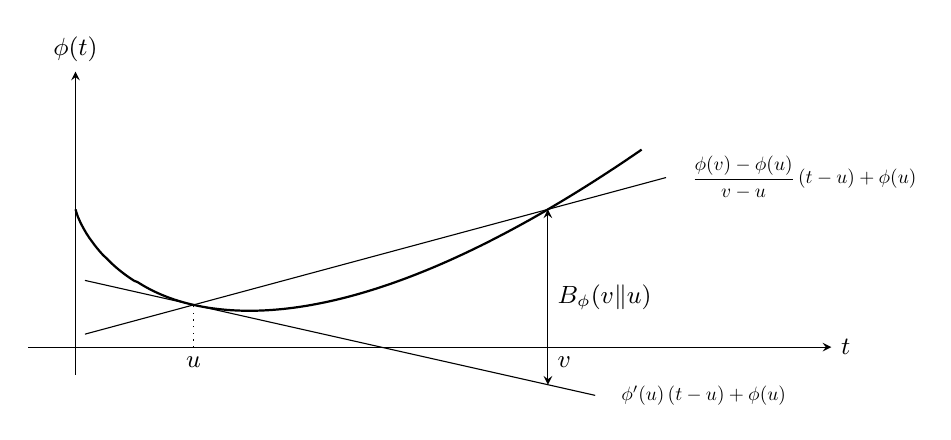
\begin{tikzpicture}
\shorthandoff{>}
%
% Concavidad de - u ln u
\begin{scope}[xscale=6,yscale=3.5]
\pgfmathsetmacro{\u}{.25};
\pgfmathsetmacro{\v}{1};
%
\draw[>=stealth,->] (-.1,-.5)--(1.6,-.5) node[right]{\small $t$};
\draw[>=stealth,->] (0,-.6)--(0,.5) node[above]{\small $\phi(t)$};
\draw[thick,domain=.005:1.2,samples=200] (0,0)-- plot (\x,{\x*ln(\x)});
\draw[dotted] (\u,-.5) node[below]{\small $u$} -- (\u,{\u*ln(\u)});
%\draw[dotted] (\v,-.55) node[below]{\small $v$} -- (\v,{\v*ln(\v)});
\draw[>=stealth,<->] (\v,{(1+ln(\u))*(\v-\u)+\u*ln(\u)}) -- (\v,{\v*ln(\v)});
\draw (\v,-.5) node[below right]{\small $v$};
\draw (\v,{.5*((1+ln(\u))*(\v-\u)+\u*ln(\u)+\v*ln(\v))}) 
node[right]{\small $B_\phi(v\|u)$};
%
\draw (.02,{(.02-\u)*(\v*ln(\v)-\u*ln(\u))/(\v-\u)+\u*ln(\u)})
-- (1.25,{(1.25-\u)*(\v*ln(\v)-\u*ln(\u))/(\v-\u)+\u*ln(\u)})
node[right,scale=.7]
{$\displaystyle \quad \frac{\phi(v)-\phi(u)}{v-u} \, (t-u) + \phi(u)$};;
%
\draw (.02,{(1+ln(\u))*(.02-\u)+\u*ln(\u)})--
(1.1,{(1+ln(\u))*(1.1-\u)+\u*ln(\u)})
node[right,scale=.7]{$\quad \phi'(u) \, (t-u) + \phi(u)$};
\end{scope}
%
%
% % Concavidad / mezcla
% \begin{scope}[xshift=8.5cm]
% \draw(0,1.25) node{\includegraphics[width=3cm]{TIKZ_SZ/DosDados}};
% \draw(-.5,2.5) node{\small $p_1$};
% \draw(1,2) node{\small $p_2$};
% \draw(2.7,1) node{\small $\lambda p_1 + (1-\lambda) p_2$};
% \draw(-.25,-1) node{\includegraphics[width=1cm]{TIKZ_SZ/Moneda}};
% \draw[>=stealth,->,thick] (-.3,-.35)--(-.75,.45);
% \draw (-.525,0) node[left]{\small $\lambda$};
% \draw[>=stealth,->,thick] (-.2,-.35)--(.3,.45);
% \draw (.05,0) node[right]{\small $1-\lambda$};
% \end{scope}
% %
% \draw (1.25,-2.25) node{(a)};
% \draw (8.25,-2.25) node{(b)};
\end{tikzpicture} \end{center}
  %
  \leyenda{$\phi$ estrictamente convexa:  la variaci\'on (cuerda) $\frac{\phi(v)
      -  \phi(u)}{v-u}$ es  mayor que  la derivada  $\phi'(u)$.  Aplicado  a dos
    distribuciones $p$ y $q$, de componentes $p_i$ y $q_i$, con $u = p_i$ y $v =
    q_i$  y  sumando, se  obtiene  $\hphi[q]  -  \hphi[p] \ge  \sum_i  (p_i-q_i)
    \phi'(p_i)$ con $\hphi \equiv H_{(\id,\phi)}, \: \id$ siendo la identidad.}
  %
  \label{Fig:SZ:ConvexidadDerivada}
  \end{figure}
  
  Aplicamos esta desigualdad a \ $u =  p_{X,Y}(x,y)$ \ y \ $v = p_X(x) p_Y(y)$ \
  y sumamos  en $x,  y$, \  para \  $(a,b) \in (  0 \,  , \,  1)^2$ \  (para que
  $C_{a,\tilde{a},b,\tilde{b}}$  \ no  sea reducido  a \  $\{0\}$), y  \  $c \in
  \mathring{C}_{a,\tilde{a},b,\tilde{b}}$ \ donde  \ $\mathring{\cdot}$ \ denota
  el interior de un conjunto, se obtiene para $\phi$ convexa,
  %
  \[
  \hphi[p_X    \otimes   p_Y]    -    \hphi[p_{X,Y}]   \:    \le    \:   c    \:
  g(a,\tilde{a},b,\tilde{b},c),
  \]
  %
  (para $\phi$  c\'oncava se  reemplaza $\hphi$ por  $-H_{-\phi}$ con  la igualdad
  inversa), donde
  %
  \begin{equation}
  g(a , \tilde{a} , b , \tilde{b} , c) = \phi'\big( a b + c \big) + \phi'\big(
  \tilde{a} \tilde{b} + c \big) - \phi'\big( a \tilde{b} - c \big) - \phi'\big(
  \tilde{a} b - c \big).
  \end{equation}
  %
  Supongamos     que    existe     un    \     $(s,\tilde{s},t,\tilde{t})    \in
  \mathring{D}_{a,\tilde{a},b,\tilde{b}}$        \        tal       que        \
  $g(s,\tilde{s},t,\tilde{t},0)  \ne  0$.   De  la continuidad  de  $\phi'$,  la
  funci\'on  $g$ es  continua,  y entonces  existe  un vecinaje  \ $V_0  \subset
  \mathring{C}_{s,\tilde{s},t,\tilde{t}}$ \ de \ $0$ \ tal que la funci\'on \ $c
  \mapsto  g(s,\tilde{s},t,\tilde{t},c)$  \ tiene  un  signo  constante sobre  \
  $V_0$.     \   Eso    permite   concluir    que    \   $c    \mapsto   c    \,
  g(s,\tilde{s},t,\tilde{t},c)$ \ no tiene un signo constante sobre \ $V_0$, \ y
  entonces de concluire que, de la  desigualdad dedibo a la concavidad de $\phi$
  (resp.   convexidad), \ $\hphi[p_{X,Y}]$  puede ser  major (resp.   menor) que
  $\hphi[p_X \otimes p_Y]$, y entonces, con la crecencia (resp.  decrecencia) de
  $h$  que  si $g(a,\tilde{a},b,\tilde{b},0)$  no  es  identicamente cero  sobre
  $\mathring{D}_{a,\tilde{a},b,\tilde{b}}$,  $\hhphi$ no  puede  ser sub-aditiva
  (distribuci\'on conjunta vs producto de las marginales).

  {\bf Etapa 2}. De la etapa  1, se sabe que la sub-aditividad es potencialmente
  posible       solamente      si       $g(a,v,s,t,0)      =       0$      sobre
  $\mathring{D}_{a,\tilde{a},b,\tilde{b}}$.  Eso   significa  que  $\phi'$  debe
  necesariamente satisfacer la ecuaci\'on funcional
  %
  \[
  \phi'\big( a  b \big)  + \phi'\big( \tilde{a}  \tilde{b} \big) -  \phi'\big( a
  \tilde{b} \big) - \phi'\big( \tilde{a} b \big) = 0,
  \]
  %
  as\'i que  no se  puede usar el  argumento de  la etapa~1 para  concluir.  Sin
  embargo,     se     puede     solucionar    esta     ecuaci\'on     funcional,
  siguiendo~\cite[\S~6]{DarJar79} donde una  ecuaci\'on funcional muy similar es
  estudiada.  Por  eso, se fija \  $(a,b) \in (0 \,  , \, 1)^2$, \  se deriva la
  identidad  precediente  con  respecto  a  \ $\tilde{a}$  \  se  multiplica  el
  resultado por $\tilde{a}$ \ para obtener
  %
  \[
  \tilde{a}  \tilde{b}   \,  \phi''(\tilde{a}   \tilde{b})  =  \tilde{a}   b  \,
  \phi''(\tilde{a} b) \qquad \mbox{para}  \qquad (\tilde{a},\tilde{b}) \in (0 \,
  , \, 1-a) \times (0 \, , \, 1-b).
  \]
  %
  Eso significa  de que $x \,  \phi''(x)$ es constante sobre  $x \in (0  \, , \,
  (1-a)  \max\{s,1-s\})$, y  para cualquier  par $(a,s)  \in (0  \, ,  \, 1)^2$.
  Entonces, $x \, \phi''(x)$ es constante sobre $x \in (0 \, , \, 1 )$, es decir
  que $\phi$ es necesariamente  de la forma $\phi(x) = \mu \, x \ln  x + \nu x +
  \vartheta$. Debido a la continuidad de $\phi$, queda v\'alido sobre el cerrado
  $[0 \, , \, 1]$.  De que se aplica a un vector de probabilidad, sumando a uno,
  se  puede  reducir  el  problema  a  $\nu =  0$  (poniendo  $\nu$  adentro  de
  $\\vartheta$  sin cambiar  el valor  de entrop\'ia  obtenida).   Adem\'as, del
  requisito $\phi(0) = 0$
  % la  constante $\vartheta$  no  altera la  concavidad  (resp. convexidad)  de
  % $\phi$, as\'i que se la puede  translatar en la funci\'on $h$ sin cambiar la
  % monotonicidad, \ie tomar
  tenemos $\vartheta =  0$.  Para que $\phi$ sea  convexa (resp. c\'oncava) hace
  falta  tener  $\mu  >  0$  (resp.   $\mu  < 0$)  as\'i  que,  sin  perdida  de
  generalidad, $\mu$ puede ser puesta tambi\'en en $h$. Tomar \ $\phi (x) = x \,
  \ln x$ \  con \ $h$ \ creciente o  \ $\phi (x) = -  x \, \ln x$ \ con  \ $h$ \
  decreciente es completamente equivalente, as\'i que se puede fijar $\phi (x) =
  x \, \ln x$ satisfaciendo la ecuaci\'on funcional, y $h$ creciente.

  En  conclusi\'on, $g  = 0$  sobre  $\mathring{D}_{a,\tilde{a},b,\tilde{b}}$ se
  reduce  a necesitar  tener $\hphi  = H$.   Esta entrop\'ia  siendo sub-aditiva
  (propidad~\ref{Prop:SZ:subaditividad}), cualquiera  funci\'on creciente de $H$
  va obviamente quedar sub-aditiva, lo que cierra la prueba.
  %
\end{proof}
%
Al rev\'es, a partir de $p_{XY}  = \frac12 \begin{bmatrix} 1 & 0 \end{bmatrix}^t
\otimes\begin{bmatrix}  1 &  0  \end{bmatrix}^t +  \frac12  \begin{bmatrix} 0  &
  1  \end{bmatrix}^t \otimes\begin{bmatrix}  0 &  1 \end{bmatrix}^t$  se obtiene
$p_X = p_Y =  \frac12 \begin{bmatrix} 1 & 1 \end{bmatrix}^t$ \  y entonces \ (i)
$\hhphi[p_{XY}]  =  h\left(  -  2  \, \phi\left(  \frac12  \right)  \right)$,  \
$\hhphi[p_X \otimes p_Y] = h\left( -  4 \, \phi\left( \frac14 \right) \right)$ \
y \ $\hhphi[p_X] + \hhphi[p_Y] = 2  \, h\left( - 2 \, \phi\left( \frac12 \right)
\right)$, \  as\'i que, en este  ejemplo \ $\hhphi[p_{XY}]  > \hhphi[p_X \otimes
p_Y]$ \ (consecuencia de la  Schur-concavidad) y \ $\hhphi[p_{XY}] > \hhphi[p_X]
+ \hhphi[p_Y]$: tampoco las $(h,\phi)$-entrop\'ia son super-aditivas.

\

La definici\'on  de entrop\'ias generalizadas condicionales  aparece mucho m\'as
problem\'atico. Por  ejemplo, si se define  a la Shannon, es  decir definiendo \
$\hhphi[X|Y]$ \ tomando \ $\sum_{y \in \Y} p_Y(y) \hhphi[p_{X|Y}(\cdot,y)]$ \ se
pierde la regla de cadena~\ref{Prop:SZ:cadena}. Como se lo ha visto, en el marco
de la entrop\'ia de Havdra-Charv\'at-Dar\'oczy se conserva la regla de cadena si
se reemplaza $p_Y$ por su potencia $p_Y^\lambda$.  Sin embargo, generalizar este
esquema en el caso general  falla (la gracia en Havdra-Charv\'at-Dar\'oczy viene
de  la  propiedad  de  morfismo  de  la  exponencial  y  del  logaritmo).   Como
consecuencia, generalizar  la noci\'on se vuelve  problem\'atico tambi\'en.  Por
ejemple  se  pierde el  diagrama  de  Venn aparte  si  se  define la  entrop\'ia
condicional  a  partir  de  la  regla  de  cadena. Pero  en  este  caso,  si  la
super-aditividad  garantiza  la positividad  de  la  entrop\'ia condicional,  se
pierde  la propiedad~\ref{Prop:SZ:independenciacondicional}  por  perdida de  la
aditividad,       y      por       consecuencia       la      propiedad       de
positividad/independencia~\ref{Prop:SZ:Ipositive}  de  una  informaci\'on  mutua
construida sobre un  modelo diagrama de Venn. Veremos  en la secci\'on siguiente
que un tercero camino puede ser usar divergencia.
% \SZ{ver con detalles \ref{Prop:SZ:condicionar} (condiconar)} \SZ{VajVas85 pour
%   la Schur-concavite}

\

Como  en  el caso  de  Shannon,  se puede  extender  la  generalizaci\'on de  la
entrop\'ia al caso de vectores  aleatorios discretos sobre de cardenal infinito,
con las mismas debilidades que en el caso de Shannon. A continuaci\'on, se puede
tambi\'en  extenderla   a  vectores   aleatorios  admitiendo  una   densidad  de
probabilidad, reemplazando la suma por una integraci\'on.

\begin{definicion}[$(h,\phi)$-entrop\'ia diferencial]
  \label{Def:SZ:HPhiEntropiaDiferencial}
  %
  Sea  $X$ una variable  aleatoria continua  sobre $\Rset^d$  y sea  $p_X(x)$ la
  densidad  (distribuci\'on)  de  probabilidad  de  $X$  de  soporte  $\X$.   La
  $(h,\phi)$-entrop\'ia diferencial de la variable $X$ es definida por
  %
  \[
  \hhphi[p_X] =  \hhphi[X] = h\left( -  \int_\X \phi\left( p_X(x)  \right) \, dx
  \right)
  \]
  %
  con  $h$  \   y  \  $\phi$  cumpliendo  los   requisitos  de  la  definici\'on
  discreta~\ref{Def:SZ:HPhiEntropia}  (de   $\phi(0)$,  se  puede   escribir  la
  integraci\'on sobre $\Rset^d$).
\end{definicion}

De nuevo  para $X =  (X_1,\ldots,X_d)$, la $(h,\phi)$-entrop\'ia  diferencial de
$X$ es una $(h,\phi)$-entrop\'ia diferencial conjunta de los $X_i$.

La  versi\'on diferencial  de la  $(h,\phi)$-entrop\'ia comparte  obviamente las
mismas debilidades  del caso particular de  Shannon: se pierden  la propiedad de
invarianza    por   transformaci\'on    biyectiva~\ref{Prop:SZ:biyeccion},   \ie
independencia       con       respecto       a       los       estados,       la
positividad~\ref{Prop:SZ:positividad},            la           de           cota
superior~\ref{Prop:SZ:cotamaxima}  (salvo  si  se  pone  v\'inculos,  ver  m\'as
adelante), en adici\'on de las que ya la versi\'on discreta perdi\'o.

Sin embargo, se conservan unas propidedades,  y entre otros si $h$ es c\'oncava,
la  $(h,\phi)$-entrop\'ia diferencia  es c\'oncava~\ref{Prop:SZ:concavidadHPhi}.
M\'as  sorprendentemente a  primer vista,  se conserva  la $(h,\phi)$-entrop\'ia
diferencial bajo un rearreglo~\ref{Prop:SZ:permutacionC},
%
\[
\hhphi[p_X^\downarrow] = \hhphi[p_X]
\]
%
\noindent De  hecho, como evocado en el  caso de Shannon, eso  fue probado entre
otros  en~\cite{LieLos01} o  \cite[Lema~7.2]{WanMad04}~\footnote{Recuerdense que
  en~\cite[Sec.~3.3]{LieLos01}  lo  muestran   para  $\phi$  diferencia  de  dos
  funciones mon\'otonas, siendo una funci\'on convexa un caso particular.}.

Se  prob\'o  en~~\cite{Cho74} o~\cite[Prop.~7.3]{WanMad04}  que  se conserva  la
Schur-concavidad~\ref{Prop:SZ:Schurconcavidad}              para             las
$\phi$-entrop\'ias.   Entonces,  de   $h$  creciente   (para   $\phi$  c\'oncava
desigualdad reversa para la integral,  pero $h$ es decreciente), se generaliza a
las $(h,\phi)$-entrop\'ias,\ie
%
\[
p  \prec q  \quad \Rightarrow  \quad \hhphi[p]  \ge \hhphi[q]  \quad  \forall \:
(h,\phi)
\]

\SZ{Quide de la reciproca? Quid sub-aditividad ssi fct creciente de Shannon?}

% ================================= Csiszar & Bregman

\subseccion{Divergencias y propiedades}
\label{Ssec:SZ:JensenBregmanCzizar}

En esta sub-secci\'on  vamos a ver que la  literatura trat\'o casi conjuntamente
de  tres  enfoques   dando  lugar  a  generalizaciones  de   la  divergencia  de
Kullback-Leibler. Lamentablemente, ninguna  generalizaci\'on contiene las otras,
a  pesar  de   que  divergencias  conocidas  pueden  partenecer   a  dos  clases
distinctas. Practicamente,  cada clase tiene  sus ventajas y  justificaci\'on en
termino de aplicaciones.


% ----- Clase de Jensen

\subsubseccion{Clase de Jensen}
\label{Sssec:SZ:Jensen}

% ----- Jensen-Shannon
%\paragraph{Primer  generalizaciones, saliendo  de Shannon  y  Kullback-Leibler -
%  divergencia de Jensen-Shannon}

Como  se lo  ha visto  tratando  de la  entrop\'ia relativa,  la divergencia  de
Kullback-Leibler no define una distancia entre distribuciones de probabilidades,
siendo no sim\'etrica  entre otros. Un primer paso  para recuperar la simetr\'ia
sin  perder  la  positividad  de  esta medida  informacional  fue  simetrizarla,
definiendo lo que es  conocido como {\it $J$-divergencia}~\cite{KulLei51, Kul68,
  Lin91}~\footnote{Esta   expresi\'on   apareci\'o  en~\cite[Ec.~(1)]{Jef46}   o
  en~\cite{Jef48},   antes   de  la   introducc\'ion   de   la  divergencia   de
  Kullback-Leibler  en el  campo de  la estimaci\'on  Bayesiana,  Jeffrey siendo
  citado por Kullback y Leibler.},
%
\[
D_J(q\|p) = \Dkl[p]{q} + \Dkl[q]{p}
\]
%
\noindent  Esta  versi\'on  simetrizada  de la  divergencia  queda  naturalmente
positiva,  pero sufre  todav\'ia  de  unas debilidades  de  $\Dkl{}$. Esta  bien
definida  siempre  que   el  soporte  de  $p$  es  incluido  en   lo  de  $q$  y
vice-versa. Adem\'as,  no cumple tampoco  la desigualdad triangular. A  pesar de
sus debilidades, se us\'o bastante en problemas de discriminaci\'on, debido a su
positividad con igualdad  si y solamente si $p = q$  (propiedad herida del hecho
de que la suma  de t\'erminos positivos es nula si y  solamente si cada uno vale
cero).

Unas decadas despu\'es, Lin  introdujo lo que llam\'o $K$-divergencia directada,
$K(p,q)   =  \Dkl[p]{\frac{p+q}{2}}$,   su  versi\'on   simetrizada,   antes  de
generalizarla    bajo     la    terminologia    de     {\it    divergencia    de
  Jensen}~\cite{Lin91}~\footnote{De  hecho, apareci\'o implicitamente  en varios
  trabajos anteriores, por ejemplo  en mecanica cu\'antica~\cite{Hol73, Hol11} o
  en reconocimiento de patrones~\cite{WonYou85}}.
%
\begin{eqnarray*}
\Djs(p_{(1)},p_{(2)})  &  = &
%
\pi_1 \Dkl[p_{(1)}]{\pi_1 p_{(1)} + \pi_2 p_{(2)}} + \pi_2 \Dkl[p_{(2)}]{\pi_1 p_{(1)} + \pi_2
  p_{(2)}}\\[2.5mm]
%
& = & H(\pi_1 p_{(1)} + \pi_2 p_{(2)}) - \pi_1 H(p_{(1)}) - \pi_2 H(p_{(2)}) \qquad \pi = [\pi_1
\quad \pi_2], \quad 0 \le \pi_1 = 1-\pi_2 \le 1
\end{eqnarray*}
%
\noindent $\Djs$ heride obviamente de  $\Dkl{}$ su positividad con igualdad si y
solamente si $p_{(1)} = p_{(2)}$.  La misma propiedad puede ser vista a trav\'es
de la desigualdad de Jensen, dando  este nombre a la medida.  Adem\'as, se quita
el problema de definici\'on, siendo de  que el soporte de $\pi_1 p_{(1)} + \pi_2
p_{(2)}$ siempre contiene  el de $p_{(1)}$ y el de  $p_{(2)}$. No es sim\'etrica
en general, pero se obtiene esta propiedad cuando $\pi = \pi_{\mathrm{u}} \equiv
[\frac12  \quad  \frac12]^t$.  Adem\'as,  en  este  caso,  a  pesar  de  que  la
divergencia   no  cumpla   la   desigualdad  triangular,   aparece  que   $\Big(
J_{\mathrm{js}}^{\pi_{\mathrm{u}}}(p_{(1)},p_{(2)})  \Big)^s, \quad  0  < s  \le
\frac12$  es una metrica~\cite{OsaBus18}  o~\cite[para $s  = \frac12$]{EndSch03,
  OstVaj03, KafOst91}.  Si puede  parecer m\'as l\'ogico definir tal divergencia
con a priori/proporciones $\pi_i$ iguales, de hecho la versi\'on no sim\'etrica,
con pesos  $\pi_i$ se vuelve  natural en el  marco de la  discriminaci\'on donde
apareci\'o implicitamente esta cantidad.  En particular, cuando estamos frente a
dos  hypotesis $i  = 1,  2$ o  clases,  a las  cuales la  distribuci\'on de  las
observaciones  es $p_{(i)}$,  con probabilidad  a priori  $\pi_i$.  A  partir de
observaciones  $x$ hay que  elegir si  eran sorteando  de $p_{(1)}$  o $p_{(2)}$
(distribuciones de  sampleos, \ie condicionalmente a la  hypotesis).  El enfoque
Bayesiano  m\'as  natural  consiste   maximizar  la  probabilidad  a  posteriori
(probabilidad de estar en hypotesis  $i$ condicionalmente a la observaci\'on), y
se prueba  que la probabilidad de  error es dada  por $P_e = \sum_x  \min( \pi_1
p_{(1)}(x)  \,  ,  \, \pi_2  p_{(2)}(x)  )$  (o  con  una  integral en  el  caso
continuo)~\cite{Kay93}. Prob\'o Lin de que
%
\[
\frac14 \left(  H_2(\pi) - \Djs(p_{(1)},p_{(2)})  \right)^2 \le P_e  \le \frac12
\left( H_2(\pi) - \Djs(p_{(1)},p_{(2)}) \right)
\]
%
con el logaritmo de base 2 en  la definici\'on de $\Djs$, lo que da naturalmente
un rol operacional a esta  divergencia.  Incidentalmente, de esta desigualdad es
inmediato ver de que $\Djs(p_{(1)},p_{(2)}) \le H_2(\pi) - 2 P_e$.  $P_e$ siendo
positivo, da
%
\[
0 \le \Djs(p_{(1)},p_{(2)}) \le  H(\pi) \le \log(2)
\]
%
\noindent (cota igual a  1 usando el logaritmo de base 2).  $\Djs$ es dicha {\it
  normalizada}.

Un otro v\'inculo  natural entre la divergencia de  Jensen-Shannon y las medidas
informacionales a la Shannon viene todav\'ia del campo de la clasificaci\'on. Si
unos datos pueden provenir de una  distribuci\'on $p_{(i)}$, $i = 1, 2$, con una
probabilidad  $\pi_i$, la variable  aleatoria $X$  dada por  los datos  tiene la
distribuci\'on  de mezcla  $p  =  \sum_i \pi_i  p_{(i)}$  como ilustrado  figura
Fig.~\ref{Fig:SZ:Concavidad}-(b).  Sea  $Z$ la variable  aleatoria binaria sobre
$\{ 1 ,  2 \}$ tal que $P(Z  = i) = \pi_i$, variable de  selecci\'on entre las
distribuciones $p_{(i)}$ (ej.   la moneda de la figura).  Por definici\'on de la
entrop\'ia  condicional,  $H(X|Z) =  \sum_i  \pi_i H(X|Z  =  i)  = \sum_i  \pi_i
H(p_{(i)})$. De  $\Djs(p_{(1)},p_{(2)}) = H(p) - \sum_i  \pi_i H(p_{(i)})$ viene
$\Djs(p_{(1)},p_{(2)}) = H(X) - H(X|Z)$, es decir
%
\[
\Djs(p_{(1)},p_{(2)}) = I(X;Z)
\]
%
La  divergencia   de  Jensen-Shannon  mide  la  informaci\'on   mutua  entre  la
observaci\'on $X$  y la variable de  selecci\'on $Z$, justificando  aun m\'as su
uso    natural   en    problemas   de    clasificaci\'on   o    selecci\'on   de
modelos. Incidentalmente, de $I(X;Z) = H(Z)  - H(Z|X) \le H(Z) \le \log(2)$ ($Z$
siendo discreta) se recupera las cotas mayor de $\Djs$.

Se  encuentran otras  desigualdades  implicando $\Djs$  y  $D_J$ o  $\Djs$ y  la
distancia  $L^1$  entre  distribuciones   o  divergencia  de  variaci\'on  total
en~\cite{Lin91}.
%~\cite{SchEla03}.

M\'as all\'a,  en el campo de la  clasificaci\'on, se puedre tratar  de m\'as de
dos  clases,   dando  lugar   a  la  generalizaci\'on   de  la   divergencia  de
Jensen-Shannon  a $n$  distribucionese probabilidad  y $\pi$  un $n$-componentes
vector de probabilidad,
%
\[
\Djs(p_{(1)},\ldots,p_{(n)})  =  H\left( \sum_i  \pi_i  p_{(i)}\right) -  \sum_i
\pi_i H(p_{(i)})
\]
%
De la  desigualdad de  Jensen, esta  cantitad queda positiva  con igualdad  si y
solamente si todos los $p_{(i)}$ son iguales. Se conserva una cota superior
%
\[
\Djs(p_{(1)},\ldots,p_{(n)}) \le H(\pi) \le \log(n)
\]
%
\noindent as\'i  que $\Djs(p_{(1)},p_{(2)}) = I(X;Z)$ con  $X$ de distribuci\'on
la mezcla $\sum_i \pi_i p_{(i)}$  y $Z$ definida sobre $\{1,\ldots,n\}$ variable
de selecci\'on de distribuci\'on $\pi$.

\SZ{convexidad?}

% ----- f-Jensen
%\paragraph{Clase de Burbea-Rao o   divergencias de Jensen}

\

Un  punto  clave  que  dio  lugar   a  la  definici\'on  de  la  divergencia  de
Jensen-Shannon es la  concavidad de la entrop\'ia de  Shannon.  Naturalmente, el
mismo enfoque  se generaliza  a cualquier entrop\'ia  c\'oncava de un  vector de
probabilidad. Tal generalizaci\'on fue  propuesta de maner formal por Burbea-Rao
e~\cite{BurRao82},  y luego  generalizado  y estudiado  m\'as detenidamente  por
Nielsen et  al.~\cite{NieBol11, NieNoc17}. A pesar  que que apareci\'o  ya en el
papel de  Burbea \& Rao,  Nielsen llam\'o tal generalizaci\'on  ``divergencia de
Burbea-Rao asimetrizada''.  M\'as formalemente, se puede definir una divergencia
de Jensen de la manera siguiente:
%
\begin{definicion}[Divergencias  de Jensen]
  Sea \ $f: \Omega  \subset \Rset^m \mapsto \Rset$ \ convexa y  de clase $C^1$ \
  sobre  \   $\Omega$,  \  un   cerrado  convexo  de   $\Rset^d$  \  y   \  $\pi
  = \begin{bmatrix} \pi_1 & \pi_2 \end{bmatrix}^t$ \ con $0 \le \pi_1 = 1-\pi_2
  \le 1$.  Las divergencias de Jensen entre dos puntos \ $u _1 , u_2 \in \Omega$
  \ son definidas por
  %
  \[
  J_f^\pi(u_1,u_2) = \pi_1 f(u_1) + \pi_2 f(u_2) - f(\pi_1 u_1 + \pi_2 u_2)
  \]
  %
  Se ilustra  a que corresponde  esta cantidad con  respecto a $f$ en  la figura
  Fig.~\ref{Fig:SZ:BregmanFJensen} m\'as adelante.
\end{definicion}
%
\noindent Esta  definici\'on se generalizada  a densidad de  probabilidad, donde
$f$  es  a  valor  reales,  actuando  sobre el  convexo  de  las  densidades  de
probabilidades~\cite{NieBol11, NieNoc17}.

Para  $(h,\phi)$-entrop\'ias \underline{c\'oncavas}  (ej.   con $h$  c\'oncava),
siendo $-\hhphi$ convexa, se puede entonces asociar una divergencia de Jensen
%
\[
\jhphi[p_{(1)}]{p_{(2)}} \equiv  J_{-\hhphi}^\pi(p_{(1)},p_{(2)}) = \hhphi[\pi_1
p_{(1)} + \pi_2 p_{(2)}] - \pi_1 \hhphi[p_{(1)}] - \pi_2 \hhphi[p_{(2)}]
\]
%
\noindent Cuando $h  \equiv \id$,  se notar\'a $\jphi{}$.

La definici\'on  se generaliza a  cualquier conjunto $\{ p_{(i)}  \}_{i=1}^n$ de
distribuciones de probabilidades y $\pi$ vector de probabilidad $n$-dimensional,
%
\[
D_{(h,\phi)}^{\mathrm{j},\pi}( \{ p_{(i)} \} ) = \hhphi[\sum_i  \pi_i p_{(i)}] -
\sum_i \pi_i \hhphi[p_{(i)}]
\]
%
\noindent Por analog\'ia a la  informaci\'on mutua, Burbea y Rao llamar\'on esta
medida ``informaci\'on mutua  generalizada''. Eso viene de que  si se define una
informaci\'on  condicional  en   el  mismo  esquema  que  el   de  Shannon,  \ie
$\hhphi[X|Y]  =  \sum_y  p_Y(y)  \hhphi[p_{X|Y}(\cdot,y)]$, entonces,  con  $\pi
\equiv p_Y$ \ y  \ $\{ p_{(i)} \}_i \equiv \{ p_{X|Y}(\cdot  , y) \}_y $ aparece
de  que  \  $D_{(h,\phi)}^{\mathrm{j},p_Y}(  \{  p_{X|Y}(\cdot ,  y)  \}_y  )  =
\hhphi[X] - \hhphi[X|Y]$.  \ Esta expresi\'on es parecida a una de las formas de
la   informaci\'on  mutua   de  Shannon,   justificando  la   terminilog\'ia  de
Burbea-Rao. Sin  embargo, hay que tener  conciencia de que no  todo se translata
obviamente  del mundo  Shannon  al  mundo generalizado.   Por  ejemplo, con  tal
definic\'on de  la entrop\'ia condicional, se  pierde la regla de  cadena, y por
consecuencia la  simetr\'ia de tal  informaci\'on mutua generalizada o  la forma
usando la entrop\'ia conjunta y las marginales.

Se  notar\'a de  que Nielsen  propus\'o generalizaciones  mas  avanzadas, usando
generalizaciones de la noci\'on  de convexidad. Estas generalizaciones van m\'as
all\'a de la meta del cap\'itulo y el lector so puede referir a~\cite{NieNoc17}.

Las divergencias de Jensen tiene las propiedades siguientes
%
\begin{enumerate}
\item Positividad:
  %
  \[
  J_f(p,q) \ge 0 \quad \mbox{con igualdad si y solamente si} \quad p = q
  \]
  %
  Esta propiedad  es la consecuencia directa  de la convexidad  estricta de $f$,
  como ilustrado figura Fig.~\ref{Fig:SZ:BregmanFJensen}.
%
  % \item  \SZ{$J_f(p,q)$  es convexa  con  respecto  al  par $(p,q)$,  pero  no
  %     necesariamente  con  respecto a  $p$  solamente  y/o  $q$. Es  tambi\'en
  %     consecuencia directa de la convexidad de $f$.}
%
\item  Pensando a  $J_f$ con  respecto a  $f$, es  lineal en  el sentido  de que
  $J_{\mu_1 f_1  + \mu_2 f_2}  = \mu_1 J_{f_1} +  \mu_2 J_{f_2}$
  (con $f_i$ convexas y $\mu_i \ge 0$).
%
  % Dualidad:  si $\phi$  tiene un  convex conjugado  $\phi^*$  (transformada de
  % Legendre)  D^{\mathrm{b}}_{\phi^*}\left(  \left.  -\nabla \hphi[q]  \right\|
  %   -\nabla \hphi[p] \right) = \bphi[q]{p}$~\cite{NieNoc17}.
%
  % Mean as minimizer: A key result about Bregman divergences is that, given a
  % random vector, the mean vector minimizes the expected Bregman divergence
  % from the random vector~\cite{FriSri08}.  This result is important because it
  % further justifies using a
  % mean as a representative of a random set, particularly in Bayesian
  % estimation.
\end{enumerate}
%
\noindent Desgraciamente,  las divergencias de Jensen no  cumplen la desigualdad
triangular  en general,  y entonces  no son  m\'etricas entre  distribuciones de
probabilidad.

Se refier\'a a~\cite{BurRao82, NieBol11, NieNoc17} para tener m\'as propiedades.

Se notar\'a que  la clase de las divergencias de Jensen  contiene el cuadrado de
la distancia de Mahalanobis (por un factor), \ie  con \ $f(u) = u^t Q u$ \ con \
$Q  > 0$ \  se obtiene  $J_f(u,v) =  \pi_1 \pi_2  (v-u)^t Q  (v-u) $  (siendo la
distancia $L^2$ un caso particular). Se generaliza al caso continuo y distancias
$L^2$ con un nucleo.
%donde $Q$ es
%una  funci\'on $\Rset^d  \times \Rset^d  \mapsto \Rset_+$  sim\'etrica definida
%positiva llamado nuclo.
%  la distancia  $L^1$  ($\displaystyle f(p)  =  \left( \int  p \right)^2$),  la
%  distancia  de Itakura-Saito  cuando  $\phi(u)  = -  \log  u$  (asociado a  la
% entrop\'ia de Burg), entre otros.


% ----- Clase de Bregman

\subsubseccion{Clase de Bregman}
\label{Sssec:SZ:Bregman}

Estas divergencias  fueron intoducidos en  el campo de la  programaci\'on lineal
convexa, para  resolver problemas de  minimizaci\'on convexa~\footnote{A\'un que
  aparece en una revista de matem\'atica y f\'isica matem\'atica, una gracia del
  papel de Bregman es que toma  el ejemplo de maximizaci\'on de la entrop\'ia de
  Shannon sujeto a momentos\ldots}~\cite{Bre67}, pero con aplicaciones en varios
campos~\cite[y ref.]{Bas89, Bas13}:
%
\begin{definicion}[Divergencias de Bregman]
  Sea \ $f: \Omega  \subset \Rset^m \mapsto \Rset$ \ convexa y  de clase $C^1$ \
  sobre  \ $\Omega$, \  un cerrado  convexo de  $\Rset^d$.  Las  divergencias de
  Bregman de  un punto  \ $v \in  \Omega$ \  relativamente a un  punto \  $u \in
  \Omega$ \ son definidas por
  %
  \[
  B_f(v\|u) = f(v) - f(u) - (v-u)^t \nabla f(u)
  \]
  %
  Dicho de otra  manera, $B_f$ corresponde al desarollo de Taylor  al orden 1 de
  $f$ en  la referencia  $u$.  Se  ilustra a que  corresponde esta  cantidad con
  respecto a $f$ en la figura Fig.~\ref{Fig:SZ:BregmanFJensen} m\'as adelante.
\end{definicion}
%
Esta  definici\'on fue generalizada  a funciones  actuando sobre  espacios m\'as
generales (ej.  actuando  sobre matrices o operadores en  espacios de Hilbert de
dimensi\'on infinita)~\cite{Pet07}.   En lo que nos concierna  en este capitulo,
tratando posiblemente de densidad de probabilidades, nos interesa a funciones de
funciones~\cite{FriSri08, NieNoc17}:
%
\begin{definicion}[Divergencias de Bregman funcional]
  Sea \ $f: \Omega \mapsto \Rset$ \ convexa y de clase $C^1$ \ sobre \ $\Omega$,
  \ un cerrado convexo de un  espacio de Banach.  Las divergencias de Bregman de
  un ``punto'' (una funci\'on) \ $v \in \Omega$ \ relativamente a un ``punto'' \
  $u \in \Omega$ \ son definidas por
  %
  \[
  B_f(v\|u) = f(v) - f(u) - \lim_{t \to 0}\frac{f( u + t (v-u) ) - f(u)}{t}
  \]
  %
  El \'ultimo t\'ermino  de esta formula es connocida  como derivada de G\^ateau
  (o derivada direccional) de $f$ en $u$ en la direcci\'on $v-u$ (siendo $u$ una
  funci\'on)~\footnote{De   hecho,   en    la   extensi\'ion   de   Frigyik   et
    al.~\cite{FriSri08}, se usa  la derivada de F\'echet, que  es m\'as general.
    Viene  de  un  l\'imite   identica  independientemente  de  la  direcci\'on.
    Entonces,  si   una  funci\'on  tiene  una  derivada   de  Fr\'echet,  tiene
    necesariamente derivadas de G\^ateau,  pero no es reciproca.  Esta subtileza
    va m\'as all\'a de la meta de esta secci\'on.}.
\end{definicion}
%
En  el  caso  de que  $\Omega  \subset  \Rset^d$  se recupera  sencillamente  la
definici\'on original.

Para  $(h,\phi)$-entrop\'ias  discretas  \underline{c\'oncavas}  (ej.   con  $h$
c\'oncava), se puede entonces asociar una divergencia de Bregman
%
\begin{eqnarray*}
\bhphi[q]{p} \equiv B_{-\hhphi}(q\|p)
& = & \hhphi[p] - \hhphi[q] - (p-q)^t \nabla \hhphi[p]\\[2.5mm]
%
%& = & \hhphi[p] - \hhphi[q] - \sum_{i=1}^n (p(x_i)-q(x_i))
% \frac{\partial}{\partial t_i} \hhphi[p]\\[2.5mm]
%
%& = & \hhphi[p] - \hhphi[q] - h'\left( \sum_j \phi(p_j) \right) \sum_i
%(p_i-q_i) \phi'(p_i)
%& = & \hhphi[p] - \hhphi[q] - h'\big(\hphi[p] \big) \sum_{i=1} (q(x)-p(x)) \phi'(p(x))
& = & \hhphi[p] - \hhphi[q] - h'\big(\hphi[p] \big) (q-p)^t \phi'(p)
\end{eqnarray*}
%
%donde    $\phi'(u)    \equiv    \begin{bmatrix}    \phi'(u_1)   &    \cdots    &
%  \phi'(u_n)  \end{bmatrix}^t$  vector  de   las  derivada  de  $\phi$  aplicada
%componente a componente.
% $t_i  \equiv p(x_i)$. 
\noindent Cuando $h \equiv \id$, se  notar\'a $\bphi{}$ y es equivalente a salir
de la  definici\'on inicial  con \ $\Omega  = [0  \, ; \,  1]$, $u$ \  y \  $v =
q(y_i)$ \ $i$-esima componente de \ $p$  \ y \ $q$ \ respectivamente, y sumar la
divergencia obtenida sobre $i$.

En el caso continuo, para las $(h,\phi)$-entrop\'ias, se obtiene
%
\[
\bhphi[q]{p} =  \hhphi[p] - \hhphi[q] -  h'\big(\hphi[p] \big) \int_\X  ( q(x) -
p(x) ) \phi'(p(x)) \, dx
\]
%
De nuevo, cuando $h \equiv \id$,  se notar\'a $\bphi{}$ y es equivalente a salir
de la  definici\'on inicial  $u =  p(x)$, \ $v  = q(x)$  y sumar  la divergencia
obtenida sobre \ $\X$.

Aparece  de  que las  divergencias  de  Jensen  se escriben  como  combinaciones
convexas de divergencias de Bregman,
%
\[
J_f^\pi(p_{(1)},p_{(2)}) = \pi_1 B_f(p_{(1)} \| \pi_1 p_{(1)} + \pi_2 p_{(2)}) +
\pi_2 \B_f(p_{(1)} \| \pi_1 p_{(1)} + \pi_2 p_{(2)})
\]
%
\noindent y vice-versa  las divergencias de Bregman se  escriben como limites de
divergencias de Jensen,
%
\[
B_f(p_{(2)}   \|  p_{(1)})   =  \lim_{\pi_2   \to  0}   \frac{J_f^\pi(p_{(1)}  ,
  p_{(2)})}{\pi_1 \pi_2}
\]
%
\noindent~\cite{Zha04, NieBol11, NieNoc17}.

La figura Fig.~\ref{Fig:SZ:BregmanFJensen} ilustra  a que corresponden \ $D_f$ \
y \ $J_f$ con respecto a la funci\'on convexa $f$.
%
\begin{figure}[h!]
%
\begin{center} \begin{tikzpicture}[xscale=8,yscale=6.5]
\shorthandoff{>}
%
\pgfmathsetmacro{\u}{.22};
\pgfmathsetmacro{\v}{1};
\pgfmathsetmacro{\al}{.65};
\pgfmathsetmacro{\mid}{\al*\u+(1-\al)*\v};
\pgfmathsetmacro{\dt}{.02}; % debut trace tangente
\pgfmathsetmacro{\ft}{1.05}; % fin trace tangente
\pgfmathdeclarefunction{sha}{1}{\pgfmathparse{#1*ln(#1)}}
\pgfmathdeclarefunction{shap}{1}{\pgfmathparse{1+ln(#1)}}
%
% Axes et f convexe (t log t ici)
\draw[>=stealth,->] (-.1,-.5)--(1.6,-.5) node[right]{\small $t$};
\draw[>=stealth,->] (0,-.7)--(0,.3) node[above]{\small $f(t)$};
\draw[thick,domain=.005:1.2,samples=199] (0,0)-- plot (\x,{sha(\x)});
%
%\draw[dotted] (\u,-.5)--(\u,{sha(\u)});
\draw (\u,-.5)--(\u,-.52) node[below]{\small $u_1$};
\draw (\v,-.5) node[below right]{\small $u_2$};
%
% ---
% tangente en u_1 y B_f(u_2 || u_1)
\draw (\dt,{shap(\u)*(\dt-\u)+sha(\u)})--(\ft,{(1+ln(\u))*(\ft-\u)+sha(\u)})
node[right,scale=.7]{$\quad f'(u_1) \, (t-u_1) + f(u_1)$};
%
\draw[>=stealth,<->] (\v,{shap(\u)*(\v-\u)+sha(\u)}) -- (\v,{sha(\v)});
\draw (\v,{.5*(shap(\u)*(\v-\u)+sha(\u)+sha(\v))}) node[right,scale=.9]{$B_f(u_2\|u_1)$};
%
% ---
% tangente en pi_1 iu_1 + pi_2 u_2
% y B_f(u_1 || pi_1 u_1 + pi_2 u_2)
%\draw[dashed] (\dt,{shap(\mid)*(\dt-\mid)+sha(\mid)})--
%(\ft,{shap(\mid)*(\ft-\mid)+sha(\mid)})
%node[right,scale=.7]{$\quad \displaystyle f'\big(\sum_i \pi_i u_i \big)
%\, \left( t-\sum_i \pi_i u_i \right) + f\left( \sum_i \pi_i u_i \right)$};
%%
%\draw[>=stealth,dashed,<->] (\v+.01,{shap(\mid)*(\v-\mid)+sha(\mid)})
% -- (\v+.01,{sha(\v)});
%\draw (\v,{.5*(shap(\mid)*(\v-\mid)+sha(\mid)+sha(\v))}) 
%node[right,scale=.7]{$B_f\big( u_1\|\sum_i \pi_i u_i \big)$};
%
% ---
% corde u_1 - u_2 et f-Jensen
\draw[dashed] (\u,{sha(\u)})--(\v,{sha(\v)});
%
\draw[>=stealth,<->] (\mid,{sha(\mid)})--(\mid,{\al*sha(\u)+(1-\al)*sha(\v)});
\draw (\mid,{.75*sha(\mid)+.25*(\al*sha(\u)+(1-\al)*sha(\v))})
node[left,scale=.85]{$J_f^\pi(u_1,u_2)$};
\draw (\mid,-.5) -- (\mid,-.52) node[below]{\small $\pi_1 u_1 + \pi_2 u_2$};
%node[right,scale=.9]{$B_f(u_2\|u_1)$};
%
\end{tikzpicture} \end{center}
%
\leyenda{$f$  estrictamente  convexa.   Las  cantidad positiva  marcada  por  la
  dupla-flecha   representan  respectivamente   la  divergencia   de  $f$-Jensen
  $J_f^\pi(u_1,u_2)$, diferencia entre la combinaci\"'on convexa de los $f(u_i)$
  y $f$ de la combinaci\'on convexa de  los $u_i$, \ y la divergencia de Bregman
  \ $B_f(u_2\|u_1)$ diferencia entre el valor en $u_2$ (punto de evaluaci\'on) y
  la  tangente  en  $u_1$  (punto  referencia). Para  $J_f^\pi$,  se  toma  como
  referencia $\pi_1 u_1 + \pi_2 u_2$, se calcula $D_f$ en los $u_i$ y se toma la
  combinaci\'on convexa.}
  %
\label{Fig:SZ:BregmanFJensen}
\end{figure}

La divergencia de Bregman tiene las propiedades siguientes
%
\begin{enumerate}
\item Positividad:
  %
  \[
  B_f(q\|p) \ge 0 \quad \mbox{con igualdad si y solamente si} \quad p = q
  \]
  %
  Esta propiedad  es la consecuencia directa  de la convexidad  estricta de $f$,
  como ilustrado figura Fig.~\ref{Fig:SZ:BregmanFJensen}.
%
\item  $B_f(q\|p)$ es convexa  con respecto  a $q$,  pero no  necesariamente con
  respecto a $p$. Es tambi\'en consecuencia directa de la convexidad de $f$.
%
\item  Pensando a  $B_f$ con  respecto a  $f$, es  lineal en  el sentido  de que
  $B_{\mu_1 f_1  + \mu_2 f_2}  = \mu_1 B_{f_1} +  \mu_2 B_{f_2}$
  (con $f_i$ convexas y $\mu_i \ge 0$).
%
  % Dualidad:  si $\phi$  tiene un  convex conjugado  $\phi^*$  (transformada de
  % Legendre)  D^{\mathrm{b}}_{\phi^*}\left(  \left.  -\nabla \hphi[q]  \right\|
  %   -\nabla \hphi[p] \right) = \bphi[q]{p}$~\cite{NieNoc17}.
%
  % Mean as minimizer: A key result about Bregman divergences is that, given a
  % random vector, the mean vector minimizes the expected Bregman divergence
  % from the random vector~\cite{FriSri08}.  This result is important because it
  % further justifies using a
  % mean as a representative of a random set, particularly in Bayesian
  % estimation.
\end{enumerate}
%
\noindent Ver~\cite{FriSri08, NieBol11, NieNoc17} para tener m\'as propiedades.

Se notar\'a que la clase de  las divergencias de Bregman contiene el cuadrado de
la distancia de Mahalanobis con \ $f(u) = u^t  Q u$ \ con \ $Q > 0$ \ (siendo la
distancia  $L^2$ un  caso particular),  el cuadrado  de la  distancia  $L^1$ con
$\displaystyle   f(u)  =  \left(   \sum_i  u_i   \right)^2$,  la   distancia  de
Itakura-Saito cuando $f(u) = - \log u$ (asociado a la entrop\'ia de Burg), entre
otros.  Unas se exteinden sencillamente al caso continuo~\cite{FriSri08}.

Como en  el caso de  divergencias de Jensen, Nielsen  propus\'o generalizaciones
m\'as avanzadas, usando las generalizaciones  de la noci\'on de convexidad usada
para generalizar  las divergencias  de Jensen. Estas  generalizaciones tambi\'en
van  m\'as all\'a  de  la  meta del  cap\'itulo  y el  lector  so puede  referir
a~\cite{NieNoc17}.

Tambi\'en,   varias  aplicaciones   se  encuentran   en   la  literatura~\cite[y
ref.]{Bas89, Csi95,  CsiMat12, Bas13}  en adici\'on de  las referencias  de esta
secci\'on, para dar unas.


% ----- Clase de Csiszar o Ali-Silvey

\subsubseccion{Clase de Csisz\'ar o Ali-Silvey}
\label{Sssec:SZ:Csiszar}

Un primer paso  generalizando la noci\'on de entrop\'ia  relativa o divergencia,
siguiendo el enfoque de Kullback  y Leibler y sus versiones tipo $J$-divergencia
o divergencia de Jensen-Shannon fue  debido a R\'enyi. En su papel~\cite{Ren61},
A. R\'enyi introdujo una noci\'on de  ganancia o perdida de informaci\'on de una
distribuci\'ion (incompleta) de probabilidad  $q$ relativa a una referencia $p$,
\  $I^\ren(q\|p)$, teniendo  un enfoque  axiom\'atico  similar al  que uso  para
definir su entrop\'ia: (i) la medida sea invariante a una misma permutaci\'on de
los componentes de $p$ y de $q$, (ii) si $\forall \, i, \: p_i \le q_i$ entonces
$I^\ren(q\|p) \ge 0$ y vice versa $I(p\|q)  \le 0$, (iii) $I([1] \| [1/2]) = 1$,
(iv)  $I( q_{(1)}  \otimes  q_{(2)} \|  p_{(1)}  \otimes p_{(2)})  =  I( q_{(1)}  \|
p_{(1)}) +  I( q_{(2)} \|  p_{(2)})$ y (v)  una propiedad de  media generalizada
$I(q_{(1)} \cup q_{(2)}  \| p_{(1)} \cup p_{(2)}) =  g^{-1} \left( \frac{w_{q_1}
    I^\ren(q_{(1)} \|  p_{(1)}) + w_{q_2} I^\ren(q_{(2)}  \| p_{(2)})}{w_{q_1} +
    w_{q_2}} \right)$ conduciendo a
%
\[
I_\lambda^\ren(q\|p)  =  \frac{1}{\lambda-1}   \log_2\left(  \sum_i  p_i  \left(
    \frac{q_i}{p_i} \right)^\lambda \right)
\]

Unos  a\~nos  despu\'es,  se introdujo  una  clase  m\'as  general debido  a  I.
Csisz\'ar~\cite{Csi63, Csi67, CsiShi04}, T.  Morimoto~\cite{Mor63} o S.  M.  Ali
\& S. D.  Silvey~\cite{AliSil66},  clase que llamaremos {\it $\phi$-divergencias
  de Csisz\`ar}. En el caso continuo toma la forma
%
\[
\cphi[q]{p} = \int_\X p(x) \phi\left( \frac{q(x)}{p(x)} \right) \, dx
\]
%
donde $\phi$ es una funci\'on convexa y  donde el soporte $\X$ de $p$ incluye lo
de $q$, y en el caso discreto una suma reemplaza la integral. Estas divergencias
o  casos particulares  fueron muy  estudiadas las  decadas que  siguieron, dando
tambi\'en  lugar  a   varias  aplicaciones~\cite{GupSha76,  BurRao82,  CreRea84,
  BenCha89, Teb92, BenBor92, SalMen93, Sal94, Csi95, CrePar00, LieVaj06}.

Como para el caso de las $\phi$-entrop\'ias, esta clase se enmarca dentro de una
clase    un     poco    m\'as    general~\cite[Secs.~4.5~\&~5]{AliSil66}    (ver
tambi\'en~\cite[Sec.~I]{OrsPar95}):
%
\begin{definicion}[$(h,\phi)$-divergencia]\label{Def:SZ:HPhiDivergencia}
  La  $(h,\phi)$-divergencia  de  una  distribuci\'on de  probabilidad  $q$  con
  respeto a una distribuci\'on $p$ de  soporte $\X$ incluyendo el soporte de $q$
  es definida por
  %
  \[
  \chphi[q]{p}  =  h\left( \sum_{x  \in  \X}  p(x) \phi\left(  \frac{q(x)}{p(x)}
    \right) \right)
  \]
  %
  en el caso discreto, y
  %
  \[
  \chphi[q]{p} =  h\left( \int_\X  p(x) \phi\left( \frac{q(x)}{p(x)}  \right) dx
  \right)
  \]
  %
  en  su versi\'on  diferencial~\footnote{En  general, por  convenci\'on, $0  \,
    \phi\left(  \frac{0}{0}  \right)  =   0$.   Adem\'as,  se  requiere  de  que
    $\displaystyle 0  \, \phi\left( \frac{a}{0} \right)  = \lim_{\varepsilon \to
      0^+} \varepsilon  \, \phi\left( \frac{a}{\varepsilon} \right)  = a \lim_{u
      \to +\infty} \frac{\phi(u)}{u}$.}, donde o
  %
  \begin{itemize}
  \item $\phi$ \ es estrictamente convexa y \ $h$ \ creciente, o
  \item $\phi$ \ es estrictamente c\'oncava y \ $h$ \ decreciente
  \end{itemize}
  %
  Frecuentemente, se supone adicionalmente que $\phi$ y $h$ son de clase $C^2$ y
  sin perdida de generalidad, que $h(\phi(1)) = 0$.
\end{definicion}
%
\noindent Se notar\'a de que, obviamente, $\cphi{} = D_{(\id,\phi)}^{\mathrm{c}}$.

Notablemente, cuando  \ $\phi(u) = u \log  u$ \ y \  $h = \id$ \  se recupera de
nuevo   la   divergencia    de   Kullback-Leibler:   esta   \'ultima   partenece
simultaneamente a la clase  de Csisz\`ar y a la de Bregman y  es la sola en este
caso~\cite{Csi91}.   Cuando \ $\phi(u)  = \pi_2  u \log  u -  (\pi_1 +  \pi_2 u)
\log(\pi_1  + \pi_2  u)$  \ y  \  $h =  \id$  \ se  recupera  la divergencia  de
Jensen-Shannon  \SZ{sola de  la clase  de Jensen  en este  caso?}.   Adem\'as de
$\Dkl{}$, la clase de Csisz\'ar contiene la ganancia de informaci\'on de R\'enyi
para  \  $\phi(u)  = u^\lambda$  \  y  \  $h(u)  = \frac{\log  u}{\lambda-1}$  \
apareciendo tambien  en una forma muy parecida  en~\cite{Hel09, Che52, CreRea84,
  LieVaj06} y  conocida como  divergencia de Chernoff  o de  Hellinger. Contiene
varias otra como la  $J$-divergencia para \ $\phi(u) = u \log u -  \log u$ \ y \
$h = \id$, la distancia de Bhattacharyya~\cite{Bha43, Bha46:07} \ $\displaystyle
-\log \int \sqrt{p  q}$ \ para \ $\phi(u) =  \sqrt{u}$ \ y \ $h(u)  = - \log u$,
instancia particular de  la de R\'enyi ($\lambda =  \frac12$), la divergencia de
variaci\'on total (o $L^1$ distancia) para $\phi(u) = |u-1|$ \ y \ $h = \id$, la
divergencia de Pearson  o divergencia $\chi^2$ para \ $\phi(u) =  (u-1)^2$ \ o \
$u^2-1$ \ y \ $h = \id$, para mencionar una.

Las divergencias de Csisz\'ar tienen las propiedades siguientes
%
\begin{enumerate}
\item Positividad:
  %
  \[
  \chphi[q]{p} \ge 0 \quad \mbox{con igualdad si y solamente si} \quad p = q
  \]
  %
  Esta propiedad es la consecuencia  directa de la convexidad estricta de $\phi$
  conjuntamente a  $h(\phi(1)) = 0$. De  hecho, de la desigualdad  de Jensen con
  $X$ de  distribuci\'on $p$ tenemos en  el caso $\phi$ convexa  y $h$ creciente
  $\chphi[q]{p}  =  h\left(   \Esp\left[  \phi\left(  \frac{q(X)}{p(X)}  \right)
    \right]  \right)  \ge  h  \left( \phi  \left(  \Esp\left[  \frac{q(X)}{p(X)}
      \right] \right)  \right) = h(\phi(1))$  (y similarmente en el  caso $\phi$
  c\'oncava  y  $h$  decreciente).  Fijense  de  que la  positividad  no  es  en
  contradicci\'on con  el enfoque  de R\'enyi en  su caso, porque  conider\'o el
  caso discreto  finito con  probabilidades incompletas, \ie  su axioma  (ii) se
  cumpla   potencialemente  solamente  para   los  vectores   de  probabilidades
  incompletos.
%
\item $\chphi{}$ satisface un teorema de  procesamiento de datos (o secunda ley de
  la  termodin\'amica)  en   el  sentido  de  que  si   dos  distribuciones  son
  consecuencias   de  la  misma   probabilidad  de   transici\'on  (condicional)
  $p_{(n+1)|(n)} = q_{(n+1)|(n)}$, entonces
  %
  \[
  \chphi[q_{(n+1)}]{p_{(n+1)}} \le \chphi[q_{(n)}]{p_{(n)}}
  \]
  \SZ{Probar}
  %
\item $\chphi{}$ es convexa con  respecto al par $(p,q)$, pero no necesariamente
  con  respecto  a  $p$  solamente  y/o  $q$. En  el  caso  $\phi$  convexa,  es
  consecuencia directa de la convexidad~\footnote{Con la hipotesis de que $\phi$
    sea  de clase $C^2$,  es sencillo  ver de  que la  Hessiana de  la funci\'on
    $(u,v) \mapsto  u \phi\left(\frac{v}{u}\right)$ con respeto a  $(u,v)$ es no
    negativa,     implicando     la     convexidad     de     esta     funci\'on
    bi-variada~\cite{CamMar09}.}   (resp.   c\'oncavidad)  de $(u,v)  \mapsto  u
  \phi\left(\frac{v}{u}\right)$ sobre  $\Rset_+^2$ conjuntamente a  la crecencia
  (resp. decrecencia) de $h$.
%
\item Pensando a $\cphi{}$  con respecto a $\phi$, es lineal en  el sentido de que
  $D_{\mu_1   \phi_1   +    \mu_2   \phi_2}^{\mathrm{c}}   =   \mu_1
  D_{\phi_1}^{\mathrm{c}}  +  \mu_2  D_{\phi_2}^{\mathrm{c}}$ (con  $\phi_i$
  convexas y $\mu_i \ge 0$).
%
\item Sea $\phi^*(u) = u \phi\left(  \frac1u \right)$. Es sencillo ver de que si
  $\phi$  es   convexa  (resp.    c\'oncava),  $\phi^*$  es   tambi\'en  convexa
  (resp.   c\'oncava).   $\phi^*$  es   llamada   {\it  $^*$-conjugada   convexa
    (resp. c\'oncava)} de $\phi$. Luego,
  %
  \[
  \chphi[q]{p} = D^{\mathrm{c}}_{(h,\phi^*)}\left( \left. p \right\| q \right)
  \]
%
\item $\chphi{}$ es  sim\'etrica si y solamente si $\phi =  \phi^* + c (\id-1)$;
  sin perdida  de generalidad, consideramos  $c = 0$.   Sin embargo, en  el caso
  general,  se  puede  definir  una   versi\'on  simetrizada  al  imagen  de  la
  $J$-divergencia,  considerando $\chphi{}  +  D^{\mathrm{c}}_{(h,\phi^*)}$.  En
  particular, cuando $h = \id$, tenemos
  %
  \[
  \cphi[q]{p}  + D^{\mathrm{c}}_{\phi^*}\left(  \left.  q \right\|  p \right)  =
  D^{\mathrm{c}}_{\phi+\phi^*}\left( \left. q \right\| p \right)
  \]
  %
  que es sim\'etrica ($(\phi^*)^* = \phi$).
%
\item Cota superior:
  %
  \[
  \chphi[q]{p} \le h\left( \phi(0) + \phi^*(0) \right)
  \]
  %
  posiblemente   infinita~\footnote{Por   ejemplo,   para  la   divergencia   de
    Kullback-Leibler,  $\phi(u) =  u \log  u$, dando  $\phi^*(u) =  - \frac{\log
      u}{u}$,  tales que  $\phi(0) =  0$ \  y \  $\phi^*(0) =  + \infty$:  no es
    acotada por arriba.}.
%
\end{enumerate}
%
\noindent  Estas  propiedades  con   varias  otras  se  encuentran  por  ejemplo
en~\cite{Vaj72,  Csi74, LieVaj87,  KafOst91, Ost96,  OstVaj03,  Vaj09, KumChi05,
  LieVaj06}.   Como en  el caso  de las  divegencias de  Jensen, en  general las
divergencias  sim\'etricas ($\phi  =  \phi^*$)  no satisfacen  en  general a  la
desigualdad  triangular,  y  entonces  no   dan  lugar  a  una  distancia  entre
distribuciones de probabilidad, aparte en casos particulares (ej. divergencia de
la  variaci\'on  total,  divergencia  de  Hellinger o  R\'enyi  con  $\lambda  =
\frac12$).      Sin     embargo,     se    prob\'o     en~\cite[Teoremas~1~\&~2,
Remark~6]{KafOst91}  \ y  \  \cite{Ost96, OstVaj03,  Vaj09}  el lema  siguiente,
condici\'on suficiente  para que una potencia  de la divergencia  satisfaga a la
desigualdad triangular:
%
\begin{lema}
  Sea \ $\phi$ \ una funci\'on convexa tal que \ $\phi^* = \phi$, \ $\phi(0) \ne
  0$   \  y   \  $\cphi{}$   su  divergencia   de  Csisz\'ar   asociada   ($h  =
  \id$).  Adicionalmente  de supone  de  que  $\phi(1)  = 0$  (ver  definici\'on
  Def.~\ref{Def:SZ:HPhiDivergencia}) y de que $\phi$ es estrictamente convexa en
  $1$.  Si existe $\kappa \in \Rset_+^*$ tal que
  %
  \[
  h(u) = \frac{\left( 1-u^\kappa  \right)^{\frac{1}{\kappa}}}{\phi(u)}, \quad u \in [ 0
  \, , \, 1) \quad \mbox{es no decreciente}
  \]
  %
  \noindent entonces
  %
  \[
  \left( \cphi[\cdot]{\cdot} \right)^s \quad s \in  (0 \, , \, \kappa] \quad \mbox{satisface
    la desigualdad triangular}
  \]
  %
  \noindent   y  entonces  es   una  m\'etrica   entre  dos   discribuciones  de
  probabilidades.
\end{lema}
%
\noindent Adem\'as, en~\cite[Sec.~3]{KafOst91} se dan condiciones necesarias que
debe cumplir $\kappa$ cuando $\phi$ tiene un comportamiento particular en $u \to
0$ \  y/o \ $u \to  0$; eso va  m\'as all\'a de la  meta de esta secci\'on  y el
lector se  podr\'a referir a~\cite{KafOst91,  Ost96, OstVaj03} para  tener m\'as
detalles.

Este   lema   se  us\'o   para   probar   el   caracter  m\'etrico   de   $\Big(
J_{\mathrm{js}}^{\pi_{\mathrm{u}}}(p_{(1)},p_{(2)})  \Big)^s, \quad  0  < s  \le
\frac12$~\cite[y   ref.]{OstVaj03,  OsaBus18},   siendo   $J_{\mathrm{js}}$  una
divergencia  de Csisz\'ar  particular.  Se  us\'o tambi\'en  para probar  de que
$\left( \cphi{}  \right)^s$ \ con \ $\phi(u)  = \frac{\lambda}{\lambda-1} \left(
  \left( 1+u^\lambda \right)^{\frac{1}{\lambda}} - 2^{\frac{1}{\lambda}-1} (1+u)
\right)$ \ y  \ $\kappa = \min\left( \lambda  \, , \, \frac12 \right)$  \ es una
m\'etrica~\cite{OstVaj03}.

% I.Csisz��r,Informationmeasures:Acriticalsurvey,In:Trans.7thPragueConf.onInformationTheory,Vol.A,1974,73����86.
% [22]
% F.Liese,I.Vajda,ConvexStatisticalDistances,In:Band95,TeubnerTextezurMathematik,Leipzig,1987.

Para  cerrar esta  secci\'on,  se  mencionar\'a de  que  varias aplicaciones  se
encuentran  en   la  literatura  que  sea   en  estimaci\'on,  discriminaci\'on,
reconocimiento de patrones, pruebas  de adecuaci\'on o inferencia estad\'istica,
entre  otros~\cite[y  ref.]{Kai67,  BoeLub79,  Poo88,  Bas89,  Csi95,  OrsPar95,
  MenMor97:5,  Par99, LieVaj06,  Par06,  NieBol11, CsiMat12, Bas13}  en  adici\'on de  las
referencias de esta secci\'on, para dar unas.

\SZ{
cf Bha 43 egalement
}


% ================================= Identidades

\subseccion{?`Como se generalizan las identidades y desigualdades?}
\label{Ssec:SZ:IdentidadesGeneralizadas}

\paragraph{Principio  de entrop\'ia m\'axima}  Si este  principio naci\'o  en el
marco de la  termodynamica o f\'isica, con la  entrop\'ia de Shannon (Boltzman),
tratando de  las nociones generalizadas de incertas,  vuelve natural preguntarse
sobre la extensi\'on  de este problema en el marco  general. \SZ{Tal estudio fue
  hecho en varios trabajos~\cite{ref, BenBor92} nous, Kesavan, Kagan 63}.

El  problema  se formaliza  como  en el  caso  Shannon,  buscando la  entrop\'ia
m\'axima  sujeto a  v\'inculos: sea  $X$ variable  aleatoria viviendo  sobre $\X
\subset \Rset^d$ con  $K$ momentos \ $\Esp\left[ M_k(X) \right]  = m_k$ \ fijos,
con $M_x: \X \to \Rset$, el problema de $(h,phi)$-entrop\'ia m\'axima se formula
de  la manera  siguiente  en el  caso continuo  (es  el caso  discreto, hay  que
re-emplazar integrales por  sumas): sean \ $M(x) = \begin{bmatrix}  1 & M_1(x) &
  \cdots & M_K(x) \end{bmatrix}^t$ \ y \ $m = \begin{bmatrix} 1 & m_1 & \cdots &
  m_K \end{bmatrix}^t$, \ se busca,
%
\[
p^* = \argmax_p \hhphi[p] \qquad \mbox{sujeto a} \qquad p \ge 0, \quad \int_\X M(x)
\, p(x) \, dx = m
\]
%
donde  los   dos  primeros  v\'inculos  aseguran  de   que  $p^*$  (positividad,
normalizaci\'on) sea  una distribuci\'on de  probabilidad. Si $\phi$  es convexa
(resp.  c\'oncava),  $h$ es creciente  (resp.  decreciente) as\'i  que maximizar
$\hhphi$ es  equivalente a maximizar $\hphi$ (resp.   $H_{-\phi}$).  Sin perdida
de generalidad, se  puede considerar la situaci\'on $\phi$  convexa.  Como en el
caso de  Shannon, introduciendo factores de Lagrange  $\mu = \begin{bmatrix}
  \mu_0  & \mu_1  & \cdots  & \mu_K  \end{bmatrix}^t$ para  tener en
cuenta    los     v\'inculos,    el    problema     variacional    consiste    a
resolver~\cite{GelFom63, Bru04, Mil00, CamMar09, CovTho06}
%
\[
p^* =  \argmax_p \int_\X \left(  - \phi\left( p(x)  \right) + \mu^t  M(x) \,
  p(x) \right) dx
\]
%
donde $\mu$ ser\'a determinado para satisfacer los v\'inculos.  De nuevo, de
la ecuaci\'on de Euler-Lagrange~\cite{GelFom63,  Bru04} se obtiene la ecuaci\'on
$-  \phi'(p(x))  + \mu^t  M(x)  = 0$.  La  funci\'on  entr\'opica $\phi$  es
c\'oncava y de  clase $C^2$, as\'i que $\phi'$ es continua  decreciente, y de la
monotonicidad es invertible. Entonces,
%
\[
p^*(x) = \phi'^{-1}\left( \mu^t M(x) \right)
\]
%
con  $\mu$  tal  que  se  satisfacen los  v\'inculos  de  normalizaci\'on  y
momentos.   Si el  resultado no  es positivo  en $\X$,  de las  condiciones KKT,
$p^*(x)  =  \Big(  \phi'^{-1}\left(  \mu^t  M(x)  \right)  \Big)_+$.   Estas
distribuci\'ones no  caen en general en  la familia exponencial.   De una forma,
usando entrop\'ia generales permite escaparse de esta familia.

Como  en el  caso de  Shannon, queda  obviamente  el hecho  de que  no se  puede
determinar $\mu$ tal que se satisfacen todos los v\'inculos (y en particular
la de normalizaci\'on).

Tal como en el caso Shannon, existe una prueba informacional:
%
\begin{lema}
  Sea \ $\displaystyle \P_m = \left\{ p \ge 0: \: \int_\X M_k(x) \, p^*(x) \, dx
    =  m \right\}$  \ y  \ $p^*  \in \P_m$  \ que  satisfaga \  $\phi'(p^*(x)) =
  \mu^t M(x)$. Entonces
  %
  \[
  \forall  \, p  \in  \P_m,  \quad \hhphi[p]  \le  \hhphi[p^*] \qquad  \mbox{con
    igualdad ssi} \quad p = p^*
  \]
  %
\end{lema}
\begin{proof}
  Sin  perdida  de  generalidad,   consideramos  $\phi$  convexa.  Calcuando  la
  divergencia de Bregman asociado a $\phi$ de $p$ relativamente a $p^*$ da
  %
  \begin{eqnarray*}
  \bphi[p]{p^*} & = & \hphi[p^*] - \hphi[p] - \int_\X \big( p(x) - p^*(x) \big)
  \, \phi'\left( p^*(x) \right) \, dx\\[2.5mm]
  %
  & = & \hphi[p^*] - \hphi[p] - \mu^t \int_\X \big( p(x) - p^*(x) \big)
  \, M(x) \, dx\\[2.5mm]
  %
  & = & \hphi[p^*] - \hphi[p]
  \end{eqnarray*}
  %
  siendo \  $p$ \ y \  $p^*$ \ en \  $\P_m$. El resulta proviene  entonces de la
  positividad de la divergencia de Bregman,  con igualdad si y solamente si $p =
  p^*$ conjuntamente a la crecencia de $h$.
\end{proof}
%
Este lema prueba que,  dando v\'inculos ``razonables'', la $(h,\phi)$-entrop\'ia
es acotada por arriba, y que se alcanza la cota. Por ejemplo,
%
\begin{itemize}
\item Con  $K =  0$ \  y \  $\X$ \ de  volumen finito  \ $|\X|  < +  \infty$, la
  distribuci\'on de $(h,\phi)$-entrop\'ia m\'axima es la distribuci\'on uniforme
  en el caso discreto tal como en el caso continuo.
%
\item \SZ{Con  $K =  1$, \ $\X  = \Rset^d$  \ y \  $M(x) = x  x^t$ (visto  con $d^2$
  v\'inculos), y $\phi(u) = u^\lambda$ (R\'enyi o Havrda-Charv\'at-Dar\'oczy), la  distribuci\'on  de  entrop\'ia  m\'axima  es \SZ{Student; Costa and son on. Gausiana se recupera caso l\'imite}.}
\end{itemize}

\

\SZ{reapparition Fisher comme courbure, cf Varma, Jizba, MenMor97...}

\SZ{EPI variaciones Madiman Barron MadBar07}

\SZ{
   On the theory  of Fisher's
  amount  of  information Sov.  Math.  Dokl., 4  (1963),  pp.  991-993, etc,  la
  codificaci\'on a la Renyi (Cambell,  Hooda 2001, Bercher) 

\

 y la cuantificacion
  fina; EPI generalizada por Madiman, etc. Lutwak, Bercher etc., Kagan; Boeke 77
  An extension  of the Fisher information  measure I. Csisz\'ar,  P. Elias (Eds.),
  Topics   in  Information  Theory,   North-Holland,  Berlin/New   York  (1977),
  pp. 113-123  o Hammad o  Vajda 73 o  Ferentinos81 en el marco  Fisher; Kesavan
  gene MaxEnt}

\SZ{Revisite capacite a la Daroczy? codage; parler de la quantification fine et HCD}
